\documentclass[aspectratio=169,xcolor=table]{beamer}
\usepackage{hyperref}
\usepackage{tikz}
\usepackage{graphicx}
\usepackage{graphbox}
\usepackage{siunitx}
\usepackage[maxcitenames=6, url=false,doi=false]{biblatex}
\usepackage{subcaption}
\usepackage[outputdir=_build,draft=false]{minted}
\usepackage{pdfpc}

\usepackage{lmodern}
\usepackage{libertine}
\renewcommand\ttdefault{lmtt}

\usepackage{dirtree}
% Unsaturated
% \definecolor{cnt}{HTML}{C7C1C2}
% \definecolor{dir}{HTML}{DBDCE8}
% \definecolor{rev}{HTML}{E7F2F2}
% \definecolor{rel}{HTML}{FFFCCD}
% \definecolor{snp}{HTML}{F5F5F5}
% \definecolor{ori}{HTML}{FFFFFF}

% Saturated, darkened
% \definecolor{cnt}{HTML}{BBA3A7}
% \definecolor{dir}{HTML}{B7BAD9}
% \definecolor{rev}{HTML}{C3E3E3}
% \definecolor{rel}{HTML}{FFF89A}
% \definecolor{snp}{HTML}{E3E3E3}
% \definecolor{ori}{HTML}{FFFFFF}

% Saturated, darkened, improved
\definecolor{cnt}{HTML}{BFA6AA}
\definecolor{dir}{HTML}{CFD2F2}
\definecolor{rev}{HTML}{C3E3E3}
\definecolor{rel}{HTML}{FFF9A3}
\definecolor{snp}{HTML}{E3E3E3}
\definecolor{ori}{HTML}{FFFFFF}

\makeatletter
\pgfkeys{/tikz/.cd,
  tab height/.initial=3pt,
  tab width/.initial=10pt,
  tab slope/.initial=1.5pt,
  cover xoff/.initial=5pt,
  cover yoff/.initial=2pt,
}
%% Note: use '\setlength{\pgf@xd}{\pgf@xb}' rather than '\pgf@xd=\pgf@xb'
%% ??? for some reason \pgf@ytt etc. didn't work, but \pgf@ytt does
\newlength\pgf@ytt
\newlength\pgf@xe
\newlength\pgf@xf
\newlength\pgf@xg
\newlength\pgf@yg
\newlength\pgf@xh
%% this didn't work
\newlength\pgf@xo  %% note: \pgf@xx is pre-defined by pgf to mean something

%% from 95.2 Communicating with the Basic Layer via Macros
% \newdimen\pgf@xta \newdimen\pgf@xtb \newdimen\pgf@ytt
% \newdimen\pgf@xoa \newdimen\pgf@xob \newdimen\pgf@yoo
\pgfdeclareshape{document}{ % or 'directory'
  %% this is nearly a rectangle
  \inheritsavedanchors[from=rectangle]
  \inheritanchorborder[from=rectangle]
  \inheritanchor[from=rectangle]{center}
  \inheritanchor[from=rectangle]{north}
  \inheritanchor[from=rectangle]{south}

  \savedmacro\tabheight{%
    \edef\tabheight{\pgfkeysvalueof{/tikz/tab height}}%
  }
  \savedmacro\tabwidth{%
    \edef\tabwidth{\pgfkeysvalueof{/tikz/tab width}}%
  }
  \savedmacro\tabslope{%
    \edef\tabslope{\pgfkeysvalueof{/tikz/tab slope}}%
  }
  \savedmacro\coverxoff{%
    \edef\coverxoff{\pgfkeysvalueof{/tikz/cover xoff}}%
  }
  \savedmacro\coveryoff{%
    \edef\coveryoff{\pgfkeysvalueof{/tikz/cover yoff}}%
  }
  %% this didn't work; probably needs \pgf@process somewhere...
  % \setlength{\pgf@xo}{\coverxoff}
  % \setlength{\pgf@xo}{0.5\pgf@xo}

  %% this didn't work either
  % \setlength{\pgf@xo}{2pt}
  % \advance\pgf@xo by \coverxoff\relax

  %% this didn't work either
  % \pgf@xx=0pt
  % \advance\pgf@xx by \coverxoff\relax
  % \pgf@xx=0.5\pgf@xx

  %% fallback, so this at least compile
  %% but moves text, because \pgf@xx is sed for node contents positioning
  % \pgf@xx=2pt % this should be 0.5 of \coverxoff

  % \inheritanchor[from=rectangle]{west}
  \anchor{west}{
    \pgf@process{\northeast}%
    \pgf@ya=.5\pgf@y%
    \pgf@process{\southwest}%
    \pgf@y=.5\pgf@y%
    % \advance\pgf@y by  \pgf@ya%
    % \advance\pgf@x by -2pt%
  }
  % \inheritanchor[from=rectangle]{east}
  \anchor{east}{%
    \pgf@process{\southwest}%
    \pgf@ya=.5\pgf@y%
    \pgf@process{\northeast}%
    \pgf@y=.5\pgf@y%
    % \advance\pgf@y by  \pgf@ya%
    % \advance\pgf@x by  2pt%
  }
  \backgroundpath{% this is new
    %% store lower left in xa/ya and upper right in xb/yb
    \southwest \pgf@xa=\pgf@x \pgf@ya=\pgf@y
    \northeast \pgf@xb=\pgf@x \pgf@yb=\pgf@y
    %% correction due to open front cover
    % \advance\pgf@xa by -2pt
    % \advance\pgf@xb by -2pt
    %%
    %% compute edges of the "divider tab" in the back cover
    %%
    \setlength{\pgf@ytt}{\pgf@yb}
    \advance\pgf@ytt by \tabheight
    \setlength{\pgf@xe}{\pgf@xa}
    \advance\pgf@xe by \tabwidth % or make it dependent on box width
    \setlength{\pgf@xf}{\pgf@xe}
    \advance\pgf@xf by \tabslope % or make it dependent on divider height
    %%
    %% compute edges of second cover of a folder ("open" cover)
    %%
    \setlength{\pgf@xg}{\pgf@xa}
    \advance\pgf@xg by \coverxoff % perhaps as an angle of open
    \setlength{\pgf@xh}{\pgf@xb}
    \advance\pgf@xh by \coverxoff
    \setlength{\pgf@yg}{\pgf@yb}
    \advance\pgf@yg by-\coveryoff % perhaps as an angle of open
    %%
    %% construct main path
    \pgfpathmoveto{\pgfpoint{\pgf@xa}{\pgf@ya}}
    \pgfpathlineto{\pgfpoint{\pgf@xa}{\pgf@ytt}}
    \pgfpathlineto{\pgfpoint{\pgf@xe}{\pgf@ytt}}
    \pgfpathlineto{\pgfpoint{\pgf@xf}{\pgf@yb}}
    \pgfpathlineto{\pgfpoint{\pgf@xb}{\pgf@yb}}
    \pgfpathlineto{\pgfpoint{\pgf@xb}{\pgf@ya}} % break for open cover
    \pgfpathmoveto{\pgfpoint{\pgf@xb}{\pgf@ya}}
    % \pfgpathlineto{\pgfpoint{\pgf@xa}{\pgf@ya}} % ??? causes error ???
    \pgfpathclose
    %% construct secondary path
    \pgfpathmoveto{\pgfpoint{\pgf@xa}{\pgf@ya}}
    % \pgfpathlineto{\pgfpoint{\pgf@xg}{\pgf@yg}}
    % \pgfpathlineto{\pgfpoint{\pgf@xh}{\pgf@yg}}
    \pgfpathlineto{\pgfpoint{\pgf@xb}{\pgf@ya}}
    \pgfpathclose
  }
}
\makeatother

% chktex-file 8
% chktex-file 36

\usetikzlibrary{calc}
\usepackage{etoolbox}

\pgfdeclarelayer{background}
\pgfdeclarelayer{foreground}
\pgfdeclarelayer{sankeydebug}
\pgfsetlayers{background,main,foreground,sankeydebug}

\newif\ifsankeydebug

\newenvironment{sankeydiagram}[1][]{

  \def\sankeyflow##1##2{% sn, en
    \path[sankey fill]
    let
    \p1=(##1.north east),\p2=(##1.south east),
    \n1={atan2(\y1-\y2, \x1-\x2)-90},
    \p3=(##2.north west),\p4=(##2.south west),
    \n2={atan2(\y3-\y4, \x3-\x4)+90}
    in
    (\p1) to[out=\n1,in=\n2] (\p3) --
    (\p4) to[in=\n1,out=\n2] (\p2) -- cycle;
    \draw[sankey draw]
    let
    \p1=(##1.north east),\p2=(##1.south east),
    \n1={atan2(\y1-\y2, \x1-\x2)-90},
    \p3=(##2.north west),\p4=(##2.south west),
    \n2={atan2(\y3-\y4, \x3-\x4)+90}
    in
    (\p1) to[out=\n1,in=\n2] (\p3)
    (\p4) to[in=\n1,out=\n2] (\p2);
  }


  \tikzset{
    sankey tot length/.store in=\sankeytotallen,
    sankey tot quantity/.store in=\sankeytotalqty,
    sankey min radius/.store in=\sankeyminradius,
    sankey arrow length/.store in=\sankeyarrowlen,
    sankey debug/.is if=sankeydebug,
    sankey debug=false,
    sankey flow/.style={
      to path={
        \pgfextra{
          \pgfinterruptpath
          \edef\sankeystart{\tikztostart}
          \edef\sankeytarget{\tikztotarget}
          \sankeyflow{\sankeystart}{\sankeytarget}
          \endpgfinterruptpath
        }
      },
    },
    sankey node/.style={
      inner sep=0,minimum height={sankeyqtytolen(##1)},
      minimum width=0,draw=none,line width=0pt,
    },
    % sankey angle
    sankey angle/.store in=\sankeyangle,
    % sankey default styles
    sankey fill/.style={line width=0pt,fill,white},
    sankey draw/.style={draw=black,line width=.4pt},
  }

  \newcommand\sankeynode[4]{%prop,orientation,name,pos
    \node[sankey node=##1,rotate=##2] (##3) at (##4) {};
    \ifsankeydebug
    \begin{pgfonlayer}{sankeydebug}
      \draw[red,|-|] (##3.north west) -- (##3.south west);
      \pgfmathsetmacro{\len}{sankeyqtytolen(##1)/3}
      \draw[red] (##3.west)
      -- ($(##3.west)!\len pt!90:(##3.south west)$)
      node[font=\tiny,text=black] {##3};
    \end{pgfonlayer}
    \fi
  }

  \newcommand\sankeynodestart[4]{%prop,orientation,name,pos
    \sankeynode{##1}{##2}{##3}{##4}
    \begin{scope}[shift={(##3)},rotate=##2]
      \path[sankey fill]
      (##3.north west) -- ++(-\sankeyarrowlen,0)
      -- ([xshift=-\sankeyarrowlen/6]##3.west)
      -- ([xshift=-\sankeyarrowlen]##3.south west)
      -- (##3.south west) -- cycle;
      \path[sankey draw]
      (##3.north west) -- ++(-\sankeyarrowlen,0)
      -- ([xshift=-\sankeyarrowlen/6]##3.west)
      -- ([xshift=-\sankeyarrowlen]##3.south west)
      -- (##3.south west);
    \end{scope}
  }

  \newcommand\sankeynodeend[4]{%prop,orientation,name,pos
    \sankeynode{##1}{##2}{##3}{##4}
    \begin{scope}[shift={(##3)},rotate=##2]
      \path[sankey fill]
      (##3.north east)
      -- ([xshift=\sankeyarrowlen]##3.east)
      -- (##3.south west) -- cycle;
      \path[sankey draw]
      (##3.north east)
      -- ([xshift=\sankeyarrowlen]##3.east)
      -- (##3.south west);
    \end{scope}
  }

  \newcommand\sankeyadvance[3][]{%newname,name,distance
    \edef\name{##2}
    \ifstrempty{##1}{
      \def\newname{##2}
      \edef\name{##2-old}
      \path [late options={name=##2,alias=\name}];
    }{
      \def\newname{##1}
    }
    \path
    let
    % sankey node angle
    \p1=(##2.north east),
    \p2=(##2.south east),
    \n1={atan2(\y1-\y2, \x1-\x2)-90},
    % sankey prop
    \p3=($(\p1)-(\p2)$),
    \n2={sankeylentoqty(veclen(\x3,\y3))},
    % next position
    \p4=($(##2.east)!##3!-90:(##2.north east)$)
    in
    \pgfextra{
      \pgfmathsetmacro{\prop}{\n2}
      \pgfinterruptpath
      \sankeynode{\prop}{\n1}{\newname}{\p4}
      \path (\name) to[sankey flow] (\newname);
      \endpgfinterruptpath
    };
  }

  \newcommand\sankeyturn[3][]{%newname,name,angle
    \edef\name{##2}
    \ifstrempty{##1}{
      \def\newname{##2}
      \edef\name{##2-old}
      \path [late options={name=##2,alias=\name}];
    }{
      \def\newname{##1}
    }
    \ifnumgreater{##3}{0}{
      \path
      let
      % sankey node angle
      \p1=(##2.north east),
      \p2=(##2.south east),
      \p3=($(\p1)!-\sankeyminradius!(\p2)$),
      \n1={atan2(\y1-\y2, \x1-\x2)-90},
      % sankey prop
      \p4=($(\p1)-(\p2)$),
      \n2={sankeylentoqty(veclen(\x4,\y4))},
      \p5=(##2.east),
      \p6=($(\p3)!1!##3:(\p5)$)
      in
      \pgfextra{
        \pgfmathsetmacro{\prop}{\n2}
        \pgfinterruptpath
        % \fill[red] (\p3) circle (2pt);
        % \fill[blue](\p6) circle (2pt);
        \sankeynode{\prop}{\n1+##3}{\newname}{\p6}
        \path (\name) to[sankey flow] (\newname);
        \endpgfinterruptpath
      };
    }{
      \path
      let
      % sankey node angle
      \p1=(##2.south east),
      \p2=(##2.north east),
      \p3=($(\p1)!-\sankeyminradius!(\p2)$),
      \n1={atan2(\y1-\y2, \x1-\x2)+90},
      % sankey prop
      \p4=($(\p1)-(\p2)$),
      \n2={sankeylentoqty(veclen(\x4,\y4))},
      \p5=(##2.east),
      \p6=($(\p3)!1!##3:(\p5)$)
      in
      \pgfextra{
        \pgfmathsetmacro{\prop}{\n2}
        \pgfinterruptpath
        % \fill[red] (\p3) circle (2pt);
        % \fill[blue](\p6) circle (2pt);
        \sankeynode{\prop}{\n1+##3}{\newname}{\p6}
        \path (\name) to[sankey flow] (\newname);
        \endpgfinterruptpath
      };
    }
  }

  \newcommand\sankeyfork[2]{%name,list of forks
    \def\name{##1}
    \def\listofforks{##2}
    \xdef\sankeytot{0}
    \path 
    let
    % sankey node angle
    \p1=(\name.north east),
    \p2=(\name.south east),
    \n1={atan2(\y1-\y2, \x1-\x2)-90},
    % sankey prop
    \p4=($(\p1)-(\p2)$),
    \n2={sankeylentoqty(veclen(\x4,\y4))}
    in
    \pgfextra{
      \pgfmathsetmacro{\iprop}{\n2}
    }
    \foreach \prop/\name[count=\c] in \listofforks {
      let
      \p{start \name}=($(\p1)!\sankeytot/\iprop!(\p2)$),
      \n{nexttot}={\sankeytot+\prop},
      \p{end \name}=($(\p1)!\n{nexttot}/\iprop!(\p2)$),
      \p{mid \name}=($(\p{start \name})!.5!(\p{end \name})$)
      in
      \pgfextra{
        \xdef\sankeytot{\n{nexttot}}
        \pgfinterruptpath
        \sankeynode{\prop}{\n1}{\name}{\p{mid \name}}
        \endpgfinterruptpath
      }
    }
    \pgfextra{
      \pgfmathsetmacro{\diff}{abs(\iprop-\sankeytot)}
      \pgfmathtruncatemacro{\finish}{\diff<0.01?1:0}
      \ifnumequal{\finish}{1}{}{
        \message{*** Warning: bad sankey fork (maybe).}
        \message{\iprop-\sankeytot}
      }
    };
  }

  \tikzset{
    % default values,
    declare function={
      sankeyqtytolen(\qty)=\qty/\sankeytotalqty*\sankeytotallen;
      sankeylentoqty(\len)=\len/\sankeytotallen*\sankeytotalqty;
    },
    sankey tot length=100pt,
    sankey tot quantity=100,
    sankey min radius=30pt,%
    sankey arrow length=10pt,%
    % user values
    #1}
}{
}

\input{../tikz/swh.tikzstyles}
\input{../tikz/swh.tikzdefs}

\definecolor{palegrey}{RGB}{242, 242, 244}
\definecolor{SwhLightRed}{cmyk}{.0,.89,.84,.07}

\setbeamercolor{background canvas}{bg=palegrey}
\useinnertheme{rounded}
\useoutertheme{shadow}
% \useoutertheme{infolines}
\usecolortheme{orchid}
\usecolortheme{whale}
\usecolortheme[named=SwhLightRed]{structure}

\setbeamerfont{footline}{series=\bfseries}
\setbeamertemplate{page number in head/foot}[totalframenumber]
\setbeamertemplate{navigation symbols}{}
\setbeamertemplate{bibliography item}[article]

\setbeamertemplate{sidebar right}{}
\setbeamertemplate{footline}{%
\insertframenumber{}/\inserttotalframenumber%
\hfill\usebeamertemplate***{navigation symbols}
\hspace{1cm}}

\rowcolors[]{1}{blue!10}{blue!05}

\setbeamertemplate{footline}
{%
  \leavevmode%
  \hbox{\begin{beamercolorbox}[wd=.5\paperwidth,ht=2.5ex,dp=1.125ex,leftskip=.3cm plus1fill,rightskip=.3cm]{author in head/foot}%
    \usebeamerfont{author in head/foot}\insertshortauthor
  \end{beamercolorbox}%
  \begin{beamercolorbox}[wd=.5\paperwidth,ht=2.5ex,dp=1.125ex,leftskip=.3cm,rightskip=.3cm plus1fil]{title in head/foot}%
    \usebeamercolor[fg]{page number in head/foot}\usebeamerfont{page number in head/foot}\usebeamertemplate{page number in head/foot}%
    \hfill%
    \usebeamerfont{title in head/foot}\insertshorttitle
  \end{beamercolorbox}}%
  \vskip0pt%
}

\titlegraphic{%
    \hfill%
    
\includegraphics[align=c, width=0.3\textwidth]{../img/frontmatter/uni_paris}%
    \hfill%
    \includegraphics[align=c, width=0.20\textwidth]{../img/frontmatter/inria.pdf}%
    \hfill%
    \includegraphics[align=c, width=0.3\textwidth]{../img/frontmatter/SWH-logo}
    \hfill%
}

\AtBeginSection[]{%
    \begin{frame}
        \frametitle{Table of Contents}
        \tableofcontents[currentsection]
    \end{frame}
}

\setbeamertemplate{headline}{}


\title[Organizing the graph of public software development]{Organizing the graph of public software development for large-scale mining}
\subtitle{PhD Thesis Defense}
\author{Antoine \textsc{Pietri}}
\institute{Inria, Paris}
\date{November 5, 2021}

\hypersetup{%
    pdfauthor={Antoine Pietri},
    pdftitle={Organizing the graph of public software development for
        large-scale mining},
    pdfkeywords={empirical software engineering, source code, open source
        software, version control system, digital preservation, graph topology,
        graph
    compression},
    pdflang={English}
}

\addbibresource{../thesis.bib}

\begin{document}
    \maketitle

    \begin{frame}{Outline}
        \tableofcontents
    \end{frame}

    \section{Introduction: Universal Mining in Software Heritage}
    % presentation
    % universal software mining

    \begin{frame}
        \frametitle{Sofware Mining}

        \begin{block}{Definition}
            \textbf{Software mining}: studying existing software to help
            improve future software development.
            % all the byproducts of software development
            % improve the software of tomorrow
            % inform development best practices
        \end{block}

        \begin{block}{Applications}
            \begin{itemize}
                \item Software health, software evolution
                \item Automated bug detection
                \item Automated vulnerability repair
                \item Code autocompletion
                \item Clone detection
                \item License compliance
                \item …
            \end{itemize}
        \end{block}
    \end{frame}

    \begin{frame}
        \frametitle{Universal Software Mining}

        \begin{block}{Current scale of software mining studies}
            \begin{itemize}
                \item Individual projects
                \item Up to thousands of popular repositories (e.g., ``top
                    1000 by stars'')
                \item Entire ecosystems (app stores, package managers, …)
            \end{itemize}
        \end{block}

        \begin{block}{Universal software mining}
            New possibilities offered by the rise of DVCS in the past 15 years.

            Next step: a framework to run empirical studies the
            \textbf{entire software commons}?

            \begin{itemize}
                \item Less repetitive, no need to crawl the data for each study
                \item Easier to replicate studies
                \item Reduce selection bias
                \item High-level view of social processes in software
                    development
            \end{itemize}
        \end{block}
    \end{frame}

    \begin{frame}
        \frametitle{In this thesis…}

        \begin{block}{}
            I study how to organize the \textbf{Software Heritage graph}, a
            comprehensive dataset of software development data, to make it
            \textbf{accessible for software mining research}.
        \end{block}

        \begin{block}{}
            \emph{End goal}: building a research platform for Universal
            Software Analysis.
            % Cite BENEVOL
        \end{block}
    \end{frame}

    \begin{frame}
        \frametitle{The Software Heritage Initiative}

        \begin{center}
            \includegraphics[width=.5\linewidth]{img/SWH-logo+motto.pdf}
        \end{center}

        \begin{block}{Collect, preserve and share \emph{all} software source
            code}
            \hfill Preserving our heritage, enabling better software and better
            science for all
            % \pause
        \end{block}

        \begin{columns}
            \begin{column}{.3\columnwidth}
                \begin{block}{Reference catalog}
                    \begin{center}
                        \includegraphics[width=.6\linewidth]{img/myriadsources}
                    \end{center}
                    \alert{find} and \alert{reference} all software source code
                    % \pause
                \end{block}
            \end{column}
            \begin{column}{.3\columnwidth}
                \begin{block}{Universal archive}
                    \begin{center}
                        \includegraphics[width=.6\linewidth]{img/fragilecloud}
                    \end{center}
                    \alert{preserve} all software source code
                    % \pause
                \end{block}
            \end{column}
            \begin{column}{.3\columnwidth}
                \begin{block}{Research infrastructure}
                    \begin{center}
                        \includegraphics[width=.7\linewidth]{img/atacama-telescope}
                    \end{center}
                    \alert{enable analysis} of all software source code
                \end{block}
            \end{column}
        \end{columns}
    \end{frame}

    \begin{frame}
        \frametitle{Data flow}
        \begin{center}
            \includegraphics[width=0.9\textwidth]{img/swh-dataflow.pdf}
        \end{center}
    \end{frame}

    \begin{frame}
        \frametitle{Archive coverage --- archive.softwareheritage.org}
        % \vspace{-1mm}
        \begin{center}
            \includegraphics[trim=0 2cm 0 0, clip, width=0.7\linewidth]{img/archive-growth.png}
        \end{center}
        % \vspace{-2mm}
        \begin{center}
            \colorbox{white}{\includegraphics[width=0.8\linewidth]{img/archive-coverage.png}}
        \end{center}
        % \pause
        \vspace{-2mm}
        \begin{block}{}
            \begin{itemize}
                \item on disk: \textasciitilde{}750 TB (uncompressed); as a
                    graph \textasciitilde{}20 B nodes, \textasciitilde{}220 B
                    edges
                \item the largest public source code archive in the world (and
                    growing!)
            \end{itemize}
        \end{block}
    \end{frame}



    \section{Data Model}

    \begin{frame}
        \frametitle{A source code directory}

        \begin{columns}
            \column{.30\textwidth}
            \begin{figure}
                \begin{minipage}{\textwidth}
                \dirtree{%
                    .1 /.
                        .2 src.
                            .3 evalexpr.c.
                            .3 parser.
                                .4 ast.c.
                                .4 parser.c.
                                .4 lexer.c.
                        .2 tests.
                            .3 eval.c.
                            .3 operands.c.
                }
            \end{minipage}
            \end{figure}
            \column{.70\textwidth}
            \begin{figure}
                \centering
                \scalebox{0.9}{\begin{tikzpicture}[scale=2, font=\footnotesize]
	\begin{pgfonlayer}{nodelayer}
		\node [style=directory] (9) at (3, -2) {};
		\node [style=directory] (10) at (1, -2) {};
		\node [style=directory] (14) at (1.5, -3) {};
		\node [style=content] (16) at (1.5, -4) {};
		\node [style=content] (17) at (2.25, -4) {};
		\node [style=content] (18) at (0.75, -4) {};
		\node [style=content] (19) at (0, -3) {};
		\node [style=directory] (20) at (2, -1.5) {};
		\node [style=content] (21) at (2.5, -3) {};
		\node [style=content] (22) at (3.5, -3) {};
	\end{pgfonlayer}
	\begin{pgfonlayer}{edgelayer}
		\draw [style=arrow] (20) to node [above,sloped] {src} (10);
		\draw [style=arrow] (10) to node [above,sloped] {evalexpr.c} (19);
		\draw [style=arrow] (10) to node [above,sloped] {parser} (14);
		\draw [style=arrow] (14) to node [above,sloped] {ast.c} (16);
		\draw [style=arrow] (14) to node [above,sloped] {lexer.c} (17);
		\draw [style=arrow] (14) to node [above,sloped] {parser.c} (18);
		\draw [style=arrow] (20) to node [above,sloped] {tests} (9);
		\draw [style=arrow] (9) to node [above,sloped] {parser.c} (21);
		\draw [style=arrow] (9) to node [above,sloped] {operands.c} (22);
	\end{pgfonlayer}
\end{tikzpicture}
}
            \end{figure}
        \end{columns}
    \end{frame}

    \begin{frame}
        \frametitle{Revisions}
        % Parallel history
        \begin{block}{}
            \begin{itemize}
                \item \textbf{Revisions} (or ``commits'') keep track of
                    successive states of a source directory.
            \end{itemize}
        \end{block}
        \vfill
        \begin{figure}
            \centering
            \scalebox{0.8}{\begin{tikzpicture}[scale=1.5, font={\small}]
	\begin{pgfonlayer}{nodelayer}
		\node [style=directory] (10) at (2, -1.5) {};
		\node [style=directory] (14) at (2, -2.25) {};
		\node [style=content] (16) at (2, -3) {};
		\node [style=content] (17) at (2.5, -3) {};
		\node [style=content] (18) at (1.5, -3) {};
		\node [style=content] (19) at (1.25, -2.25) {};
		\node [style=directory] (20) at (2, -0.75) {};
		\node [style=revision, label={[align=center]\textbf{Second revision} \\ Add parser}] (23) at (2, 0) {};
		\node [style=revision, label={[align=center]\textbf{Third revision} \\ Add tests}] (24) at (5, 0) {};
		\node [style=directory] (25) at (5.5, -1.5) {};
		\node [style=directory] (26) at (4.5, -1.5) {};
		\node [style=directory] (27) at (4.5, -2.25) {};
		\node [style=content] (28) at (4.5, -3) {};
		\node [style=content] (29) at (5, -3) {};
		\node [style=content] (30) at (4, -3) {};
		\node [style=content] (31) at (3.75, -2.25) {};
		\node [style=directory] (32) at (5, -0.75) {};
		\node [style=content] (33) at (5.25, -2.25) {};
		\node [style=content] (34) at (5.75, -2.25) {};
		\node [style=revision, label={[align=center]\textbf{First revision} \\ Initial prototype}] (35) at (-1, 0) {};
		\node [style=directory] (36) at (-1, -0.75) {};
		\node [style=content] (37) at (-1, -1.5) {};
		\node [style=none] (38) at (-1, 1.5) {};
		\node [style=none] (39) at (5, 1.5) {};
	\end{pgfonlayer}
	\begin{pgfonlayer}{edgelayer}
		\draw [style=arrow] (10) to (14);
		\draw [style=arrow] (14) to (16);
		\draw [style=arrow] (14) to (17);
		\draw [style=arrow] (20) to node [above, sloped] {\tiny src} (10);
		\draw [style=arrow] (10) to (19);
		\draw [style=arrow] (14) to (18);
		\draw [style=arrow] (23) to (20);
		\draw [style=arrow] (24) to (23);
		\draw [style=arrow] (26) to (27);
		\draw [style=arrow] (27) to (28);
		\draw [style=arrow] (27) to (29);
		\draw [style=arrow] (32) to node [above, sloped] {\tiny src} (26);
		\draw [style=arrow] (32) to node [above, sloped] {\tiny tests} (25);
		\draw [style=arrow] (26) to (31);
		\draw [style=arrow] (27) to (30);
		\draw [style=arrow] (25) to (33);
		\draw [style=arrow] (25) to (34);
		\draw [style=arrow] (24) to (32);
		\draw [style=arrow] (23) to (35);
		\draw [style=arrow] (35) to (36);
		\draw [style=arrow] (36) to (37);
		\draw [style=arrow] (38.center) to node [above] {Time} (39.center);
	\end{pgfonlayer}
\end{tikzpicture}
}
        \end{figure}
    \end{frame}

    \begin{frame}
        \frametitle{Branching and merging}

        \begin{block}{}
            \begin{itemize}
                \item ``Branching'' allows multiple developers to work on
                    different features simultaneously.
                \item ``Merging'' is used to integrate their respective changes
                    back to a shared state.
            \end{itemize}
        \end{block}
        \vfill
        \begin{figure}
            \centering
            \scalebox{0.8}{\begin{tikzpicture}
	\begin{pgfonlayer}{nodelayer}
		\node [style=revision] (0) at (0, 0) {};
		\node [style=revision, label={[align=center]below:Branching\\revision}] (1) at (2, 0) {};
		\node [style=revision] (2) at (4, 0) {};
		\node [style=revision] (3) at (3, 1) {};
		\node [style=revision] (4) at (4.75, 1) {};
		\node [style=revision] (5) at (6, 0) {};
		\node [style=revision, label={[align=center]below:Merge\\revision}] (6) at (8, 0) {};
		\node [style=revision] (7) at (6.5, 1) {};
		\node [style=revision] (8) at (9.5, 0) {};
	\end{pgfonlayer}
	\begin{pgfonlayer}{edgelayer}
		\draw [style=arrow] (1) to (0);
		\draw [style=arrow] (3) to (1);
		\draw [style=arrow] (4) to (3);
		\draw [style=arrow] (7) to (4);
		\draw [style=arrow] (6) to (7);
		\draw [style=arrow] (2) to (1);
		\draw [style=arrow] (5) to (2);
		\draw [style=arrow] (6) to (5);
		\draw [style=arrow] (8) to (6);
	\end{pgfonlayer}
\end{tikzpicture}
}
        \end{figure}
    \end{frame}

    \begin{frame}
        \frametitle{Branches}
        \begin{block}{}
            \begin{itemize}
                \item \textbf{Branches} are dynamic pointers to revisions,
                    using mnemonic names to keep track of their purpose.
                \item Branch pointers move when more revisions are added to the
                    branch.
            \end{itemize}
        \end{block}
        % TODO: animate
        \vfill
        \begin{figure}
            \centering
            \scalebox{0.8}{\begin{tikzpicture}
	\begin{pgfonlayer}{nodelayer}
		\node [style=revision] (0) at (0, 0) {};
		\node [style=revision] (1) at (2, 0) {};
		\node [style=revision] (2) at (4, 0) {};
		\node [style=revision] (3) at (6, 0) {};
		\node [style=revision] (4) at (8, 0) {};
		\node [style=revision] (5) at (3, 1) {};
		\node [style=revision] (6) at (5, 1) {};
		\node [style=revision] (7) at (5, -1) {};
		\node [style=revision] (8) at (7, -1) {};
		\node [style=branch] (9) at (5, 2.25) {feature-parser};
		\node [style=branch] (10) at (8, 2.25) {main};
		\node [style=branch] (11) at (9, 1) {test-ci};
		\node [style=revision] (12) at (9, -1) {};
	\end{pgfonlayer}
	\begin{pgfonlayer}{edgelayer}
		\draw [style=arrow] (1) to (0);
		\draw [style=arrow] (2) to (1);
		\draw [style=arrow] (3) to (2);
		\draw [style=arrow] (4) to (3);
		\draw [style=arrow] (5) to (1);
		\draw [style=arrow] (6) to (5);
		\draw [style=arrow] (7) to (2);
		\draw [style=arrow] (8) to (7);
		\draw [style=dashed arrow] (9) to (6);
		\draw [style=dashed arrow] (10) to (4);
		\draw [style=dashed arrow] (11) to (12);
		\draw [style=arrow] (12) to (8);
	\end{pgfonlayer}
\end{tikzpicture}
}
        \end{figure}
    \end{frame}

    \begin{frame}
        \frametitle{Releases}
        \begin{block}{}
            \begin{itemize}
                \item \textbf{Releases} (or ``tags'') point to specific
                    milestones in the development history.
                \item They have mnemonic names, usually representing the
                    software version.
            \end{itemize}
        \end{block}
        % TODO: animate
        \vfill
        \begin{figure}
            \centering
            \scalebox{0.8}{\begin{tikzpicture}
	\begin{pgfonlayer}{nodelayer}
		\node [style=revision] (0) at (0, 0) {};
		\node [style=revision] (1) at (2, 0) {};
		\node [style=revision] (2) at (4, 0) {};
		\node [style=revision] (3) at (6, 0) {};
		\node [style=revision] (4) at (8, 0) {};
		\node [style=revision] (7) at (3, -1) {};
		\node [style=revision] (8) at (5, -1) {};
		\node [style=branch] (10) at (10, 2) {main};
		\node [style=revision] (12) at (7, -1) {};
		\node [style=revision] (13) at (10, 0) {};
		\node [style=revision] (14) at (6, -2) {};
		\node [style=revision] (15) at (8, -2) {};
		\node [style=release, label={\textbf{v2.0}}] (16) at (8, 2) {};
		\node [style=release, label={\textbf{v1.0}}] (17) at (4, 2) {};
	\end{pgfonlayer}
	\begin{pgfonlayer}{edgelayer}
		\draw [style=arrow] (1) to (0);
		\draw [style=arrow] (2) to (1);
		\draw [style=arrow] (3) to (2);
		\draw [style=arrow] (4) to (3);
		\draw [style=arrow] (8) to (7);
		\draw [style=arrow] (12) to (8);
		\draw [style=arrow] (4) to (12);
		\draw [style=arrow] (7) to (1);
		\draw [style=dashed arrow] (10) to (13);
		\draw [style=arrow] (13) to (4);
		\draw [style=arrow] (14) to (8);
		\draw [style=arrow] (15) to (14);
		\draw [style=dashed arrow] (16) to (4);
		\draw [style=dashed arrow] (17) to (2);
	\end{pgfonlayer}
\end{tikzpicture}
}
        \end{figure}
    \end{frame}

    \begin{frame}
        \frametitle{Deduplication}
        \begin{block}{}
            \begin{itemize}
                \item Lots of frozen states $\Rightarrow$ lots of copies of
                    objects
                \item Most objects stay identical from one revision to another
                \pause
                \item We can identify \& deduplicate them with
                    \textbf{cryptographic hash functions}.
            \end{itemize}
        \end{block}
        \vfill
        \begin{figure}
            \centering
            \scalebox{0.8}{\begin{tikzpicture}
    \node [
        shape=rectangle, draw=black, align=left, font=\tiny,
        label={[above]Input text}
    ] (input) at (0, 0)
        {%
            L'argoumante était églomatique et s'impliquait \\
            beaucoup plus qu'à l'exparité. Le plus déjà se \\
            plussissait. Plus qu'à l'exparité s'étrangent et se \\
            consument les pregmes endiablés de la légume.
    };

    \node [
        shape=ellipse, draw=black, align=left, fill=cyan!25,
        label={[above,align=center]Cryptographic \\ hash function}
    ] (hash) at (5.5, 0) {SHA-256};

    \node [
        shape=rectangle, draw=black, align=center, font=\footnotesize,
        label={[above]Result hash}
    ] (output) at (10, 0) {%
        % \texttt{7a50e30ada8f09b2}%
        % \texttt{24d348d314de4c09} \\
        % \texttt{ae0ebcb443334442}%
        % \texttt{70cc832ebfc6bc0c}

        \texttt{7a50e30ada8f09b224d34} \\
        \texttt{8d314de4c09ae0ebcb443} \\
        \texttt{33444270cc832ebfc6bc0c}
    };

    \draw[->, >=Stealth] (input) to (hash);
    \draw[->, >=Stealth] (hash) to (output);
\end{tikzpicture}
}
        \end{figure}
        \begin{block}{Cryptographic hash functions (SHA-1, SHA-256, BLAKE2, …)}
            \begin{itemize}
                \item Associates an arbitrary input with a
                    \emph{unique\footnote{Terms and conditions apply.}
                    identifier} called a \textbf{hash}
                \item Check if two objects are identical in O(1).
            \end{itemize}
        \end{block}
    \end{frame}

    \begin{frame}
        \frametitle{Deduplicating files}
        \begin{block}{}
            \begin{itemize}
                \item VCSs identify each file via their unique hash
                \item Identical files are \emph{deduplicated} (= shared) from
                    one revision to another.
            \end{itemize}
        \end{block}
        % TODO: animate
        \vfill
        \begin{figure}
            \centering
            \scalebox{0.8}{\begin{tikzpicture}[scale=1.5, font={\small}]
	\begin{pgfonlayer}{nodelayer}
		\node [style=directory] (10) at (2, -1.5) {};
		\node [style=directory] (14) at (2, -2.25) {};
		\node [style=content] (16) at (2, -3.5) {C};
		\node [style=content] (17) at (2.5, -3.5) {D};
		\node [style=content] (18) at (1.5, -3.5) {B};
		\node [style=content, fill=white, dotted] (19) at (1.25, -2.25) {A};
		\node [style=directory] (20) at (2, -0.75) {};
		\node [style=revision] (23) at (2, 0) {};
		\node [style=revision] (24) at (5, 0) {};
		\node [style=directory] (25) at (5.5, -1.5) {};
		\node [style=directory] (26) at (4.5, -1.5) {};
		\node [style=directory] (27) at (4.5, -2.25) {};
		\node [style=content, fill=white, dotted] (28) at (4.5, -3.5) {C};
		\node [style=content, fill=white, dotted] (29) at (5, -3.5) {D};
		\node [style=content, fill=white, dotted] (30) at (4, -3.5) {B};
		\node [style=content, fill=white, dotted] (31) at (3.75, -2.25) {A};
		\node [style=directory] (32) at (5, -0.75) {};
		\node [style=content] (33) at (5.25, -2.25) {E};
		\node [style=content] (34) at (5.75, -2.25) {F};
		\node [style=revision] (35) at (-1, 0) {};
		\node [style=directory] (36) at (-1, -0.75) {};
		\node [style=content] (37) at (-1, -1.5) {A};
	\end{pgfonlayer}
	\begin{pgfonlayer}{edgelayer}
		\draw [style=arrow] (10) to (14);
		\draw [style=arrow] (14) to (16);
		\draw [style=arrow] (14) to (17);
		\draw [style=arrow] (20) to node [above, sloped] {\tiny src} (10);
		\draw [style=dashed arrow, dotted] (10) to (19);
		\draw [style=arrow] (14) to (18);
		\draw [style=arrow] (23) to (20);
		\draw [style=arrow] (24) to (23);
		\draw [style=arrow] (26) to (27);
		\draw [style=dashed arrow, dotted] (27) to (28);
		\draw [style=dashed arrow, dotted] (27) to (29);
		\draw [style=arrow] (32) to node [above, sloped] {\tiny src} (26);
		\draw [style=arrow] (32) to node [above, sloped] {\tiny tests} (25);
		\draw [style=dashed arrow, dotted] (26) to (31);
		\draw [style=dashed arrow, dotted] (27) to (30);
		\draw [style=arrow] (25) to (33);
		\draw [style=arrow] (25) to (34);
		\draw [style=arrow] (24) to (32);
		\draw [style=arrow] (23) to (35);
		\draw [style=arrow] (35) to (36);
		\draw [style=arrow] (36) to (37);
		\draw [style=red arrow, bend left=15] (10) to (37);
		\draw [style=red arrow, bend left=15, looseness=0.75] (26) to (37);
		\draw [style=red arrow, in=-300, out=-135, looseness=0.75] (27) to (18);
		\draw [style=red arrow, in=75, out=-135, looseness=0.75] (27) to (16);
		\draw [style=red arrow, in=75, out=-135] (27) to (17);
	\end{pgfonlayer}
\end{tikzpicture}
}
        \end{figure}
    \end{frame}

    \begin{frame}
        \frametitle{Deduplicating directories}
        \begin{block}{}
            \begin{itemize}
                \item Similarly, directories can be identified by a unique hash
                \item Recursively computed from their entire subtree
                \item Identical directories are also deduplicated across
                    revisions
            \end{itemize}
        \end{block}
        % TODO: animate
        \vfill
        \begin{figure}
            \centering
            \scalebox{0.8}{\begin{tikzpicture}[scale=1.5, font={\small}]
	\begin{pgfonlayer}{nodelayer}
		\node [style=directory] (10) at (2, -1.5) {3};
		\node [style=directory] (14) at (2, -2.25) {4};
		\node [style=content] (16) at (2, -3.5) {C};
		\node [style=content] (17) at (2.5, -3.5) {D};
		\node [style=content] (18) at (1.5, -3.5) {B};
		\node [style=content, fill=white, dotted] (19) at (1.25, -2.25) {A};
		\node [style=directory] (20) at (2, -0.75) {2};
		\node [style=revision] (23) at (2, 0) {};
		\node [style=revision] (24) at (4.25, 0) {};
		\node [style=directory] (25) at (4.75, -1.5) {6};
		\node [style=directory, fill=white, dotted] (26) at (3.75, -1.5) {3};
		\node [style=directory, fill=white, dotted] (27) at (3.75, -2.25) {4};
		\node [style=content, fill=white, dotted] (28) at (3.75, -3.5) {C};
		\node [style=content, fill=white, dotted] (29) at (4.25, -3.5) {D};
		\node [style=content, fill=white, dotted] (30) at (3.25, -3.5) {B};
		\node [style=content, fill=white, dotted] (31) at (3, -2.25) {A};
		\node [style=directory] (32) at (4.25, -0.75) {5};
		\node [style=content] (33) at (4.5, -2.25) {E};
		\node [style=content] (34) at (5, -2.25) {F};
		\node [style=revision] (35) at (0.25, 0) {};
		\node [style=directory] (36) at (0.25, -0.75) {1};
		\node [style=content] (37) at (0.25, -2.25) {A};
	\end{pgfonlayer}
	\begin{pgfonlayer}{edgelayer}
		\draw [style=arrow] (10) to (14);
		\draw [style=arrow] (14) to (16);
		\draw [style=arrow] (14) to (17);
		\draw [style=arrow] (20) to node [above, sloped] {\tiny src} (10);
		\draw [style=dashed arrow, dotted] (10) to (19);
		\draw [style=arrow] (14) to (18);
		\draw [style=arrow] (23) to (20);
		\draw [style=arrow] (24) to (23);
		\draw [style=dashed arrow, dotted] (26) to (27);
		\draw [style=dashed arrow, dotted] (27) to (28);
		\draw [style=dashed arrow, dotted] (27) to (29);
		\draw [style=dashed arrow, dotted] (32) to node [above, sloped, color={black!60}] {\tiny src} (26);
		\draw [style=arrow] (32) to node [above, sloped] {\tiny tests} (25);
		\draw [style=dashed arrow, dotted] (26) to (31);
		\draw [style=dashed arrow, dotted] (27) to (30);
		\draw [style=arrow] (25) to (33);
		\draw [style=arrow] (25) to (34);
		\draw [style=arrow] (24) to (32);
		\draw [style=arrow] (23) to (35);
		\draw [style=arrow] (35) to (36);
		\draw [style=arrow] (36) to (37);
		\draw [style=red arrow, bend right=15] (10) to (37);
		\draw [style=red arrow] (32) to node [above, sloped, color={red!70!black}] {\tiny src} (10);
	\end{pgfonlayer}
\end{tikzpicture}
}
        \end{figure}
    \end{frame}

    \begin{frame}
        \frametitle{Merkle DAG}
        \begin{block}{}
            \begin{itemize}
                \item Hash-based deduplication applied on every node in the graph
                    $\Rightarrow$ \textbf{Merkle DAG}
                \item Saves space, ensures data integrity
                \item Persistent structure, never rewrites nodes, great for
                    archival
                \item Changing a single object only requires
                    $O(h)$ new nodes
            \end{itemize}
        \end{block}
        \vfill
        \begin{figure}
            \centering
            \scalebox{0.8}{\begin{tikzpicture}[scale=1.5, font={\small}]
	\begin{pgfonlayer}{nodelayer}
		\node [style=directory] (10) at (1.5, -1.5) {};
		\node [style=directory] (14) at (1.5, -2.25) {};
		\node [style=content] (16) at (1.25, -3.25) {C};
		\node [style=content] (17) at (1.75, -3.25) {D};
		\node [style=directory] (20) at (2, -0.75) {};
		\node [style=revision] (23) at (2, 0) {};
		\node [style=revision] (24) at (6, 0) {};
		\node [style=directory] (25) at (2.5, -1.5) {};
		\node [style=directory] (29) at (2.5, -2.25) {};
		\node [style=directory] (30) at (3.25, -2.25) {};
		\node [style=content] (31) at (2.75, -3.25) {F};
		\node [style=content] (32) at (3.25, -3.25) {G};
		\node [style=content] (33) at (3.75, -3.25) {H};
		\node [style=directory] (37) at (6, -0.75) {};
		\node [style=directory] (38) at (6, -1.5) {};
		\node [style=directory] (39) at (6, -2.25) {};
		\node [style=content] (40) at (6, -3.25) {H'};
		\node [style=directory] (42) at (0.75, -2.25) {};
		\node [style=content] (43) at (2.25, -3.25) {E};
		\node [style=content] (44) at (0.75, -3.25) {B};
		\node [style=content] (45) at (0.25, -3.25) {A};
	\end{pgfonlayer}
	\begin{pgfonlayer}{edgelayer}
		\draw [style=arrow] (10) to (14);
		\draw [style=arrow] (14) to (16);
		\draw [style=arrow] (14) to (17);
		\draw [style=arrow] (20) to (10);
		\draw [style=arrow] (24) to (23);
		\draw [style=arrow] (25) to (29);
		\draw [style=arrow] (29) to (31);
		\draw [style=arrow] (30) to (32);
		\draw [style=arrow] (10) to (42);
		\draw [style=arrow] (42) to (44);
		\draw [style=arrow] (42) to (45);
		\draw [style=arrow] (29) to (43);
		\draw [style=arrow, in=-315, out=-150, looseness=1.25] (38) to (29);
		\draw [style=arrow, in=-300, out=-150, looseness=1.25] (39) to (32);
		\draw [style=arrow, in=-330, out=-150, looseness=1.25] (37) to (10);
		\draw [style=red arrow] (20) to (25);
		\draw [style=red arrow] (25) to (30);
		\draw [style=red arrow] (23) to (20);
		\draw [style=red arrow] (30) to (33);
		\draw [style=red arrow] (24) to (37);
		\draw [style=red arrow] (37) to (38);
		\draw [style=red arrow] (38) to (39);
		\draw [style=red arrow] (39) to (40);
		\draw [decorate, decoration={brace,raise=20pt,amplitude=10pt}] (24) to node [right=35pt, style=none] {$h$} (40);
	\end{pgfonlayer}
\end{tikzpicture}
}
        \end{figure}
    \end{frame}

    \begin{frame}
        \frametitle{Consolidation in a single archive}

        \begin{columns}
            \column{.40\textwidth}
            \begin{block}{}
                \begin{itemize}
                    \item In Software Heritage, \emph{all} the repositories are
                        consolidated in a single archive
                    \item Software artifacts are deduplicated \emph{across
                        different repositories}
                    \item The result is a single graph containing \textbf{all
                        the software artifacts in our software commons}.
                    \item Helpful analogy: like a single Git repository but
                        with all the public code in the world.
                \end{itemize}
            \end{block}
            \column{.60\textwidth}
            \begin{figure}
                \centering
                \scalebox{0.5}{\begin{tikzpicture}[scale=1.3, font={\tiny}, {every node/.style}={scale=1}]
	\begin{pgfonlayer}{nodelayer}
		\node [style=directory] (10) at (2, -3.5) {3};
		\node [style=content] (14) at (2, -4.25) {B};
		\node [style=directory] (20) at (1.5, -2.75) {2};
		\node [style=revision] (23) at (1.5, -2) {$\beta$};
		\node [style=revision] (24) at (2.5, -2) {$\gamma$};
		\node [style=directory] (25) at (3, -3.5) {6};
		\node [style=directory] (32) at (2.5, -2.75) {5};
		\node [style=content] (33) at (2.75, -4.25) {C};
		\node [style=content] (34) at (3.5, -4.25) {D};
		\node [style=revision] (35) at (0.5, -2) {$\alpha$};
		\node [style=directory] (36) at (0.5, -2.75) {1};
		\node [style=content] (37) at (1.25, -4.25) {A};
		\node [style=none] (38) at (0, 0) {};
		\node [style=none] (39) at (4, 0) {};
		\node [style=none] (40) at (4, -4.75) {};
		\node [style=none] (41) at (0, -4.75) {};
		\node [style=release] (42) at (2.75, -1.25) {y};
		\node [style=directory] (43) at (2, -9.25) {3};
		\node [style=content] (44) at (2, -10) {B};
		\node [style=directory] (48) at (1.5, -8.5) {2};
		\node [style=revision] (49) at (1.5, -7.75) {$\beta$};
		\node [style=revision] (50) at (2.5, -7.75) {$\gamma'$};
		\node [style=directory] (51) at (3, -9.25) {6'};
		\node [style=directory] (52) at (2.5, -8.5) {5'};
		\node [style=content] (53) at (2.75, -10) {C};
		\node [style=content] (54) at (3.5, -10) {D'};
		\node [style=revision] (55) at (0.5, -7.75) {$\alpha$};
		\node [style=directory] (56) at (0.5, -8.5) {1};
		\node [style=content] (57) at (1.25, -10) {A};
		\node [style=none] (58) at (0, -5.75) {};
		\node [style=none] (59) at (4, -5.75) {};
		\node [style=none] (60) at (4, -10.5) {};
		\node [style=none] (61) at (0, -10.5) {};
		\node [style=release] (62) at (2.75, -7) {y'};
		\node [style=release] (63) at (1.5, -1.25) {x};
		\node [style=release] (64) at (1.5, -7) {x};
		\node [style=directory] (65) at (8.25, -6.5) {3};
		\node [style=content] (66) at (8.25, -7.25) {B};
		\node [style=directory] (70) at (7.75, -5.75) {2};
		\node [style=revision] (71) at (7.75, -5) {$\beta$};
		\node [style=revision] (72) at (8.75, -4.25) {$\gamma$};
		\node [style=directory] (73) at (9.25, -6.5) {6};
		\node [style=directory] (74) at (8.75, -5.75) {5};
		\node [style=content] (75) at (9, -7.25) {C};
		\node [style=content] (76) at (9.75, -7.25) {D};
		\node [style=revision] (77) at (6.75, -5) {$\alpha$};
		\node [style=directory] (78) at (6.75, -5.75) {1};
		\node [style=content] (79) at (7.5, -7.25) {A};
		\node [style=release] (80) at (8.75, -3.25) {y};
		\node [style=release] (81) at (7.75, -4.25) {x};
		\node [style=revision] (82) at (10, -5) {$\gamma'$};
		\node [style=release] (83) at (10, -3.25) {y'};
		\node [style=directory] (84) at (10, -5.75) {5'};
		\node [style=directory] (85) at (10.25, -6.5) {6'};
		\node [style=content] (87) at (10.75, -7.25) {D'};
		\node [style=none] (88) at (6, -1.75) {};
		\node [style=none] (89) at (11.5, -1.75) {};
		\node [style=none] (90) at (11.5, -8) {};
		\node [style=none] (91) at (6, -8) {};
		\node [style=snapshot] (92) at (2, -6.25) {SNP-2};
		\node [style=snapshot] (93) at (2, -0.5) {SNP-1};
		\node [style=snapshot] (94) at (7, -2.25) {SNP-1};
		\node [style=snapshot] (95) at (9, -2.25) {SNP-2};
		\node [style=none] (96) at (4, -2.5) {};
		\node [style=none] (97) at (4, -8.25) {};
		\node [style=none] (98) at (6, -4) {};
		\node [style=none] (99) at (6, -6) {};
		\node [style=none] (100) at (5, -5.25) {\normalsize \emph{Ingestion}};
	\end{pgfonlayer}
	\begin{pgfonlayer}{edgelayer}
		\draw [style=arrow] (10) to (14);
		\draw [style=arrow] (20) to (10);
		\draw [style=arrow] (23) to (20);
		\draw [style=arrow] (24) to (23);
		\draw [style=arrow] (32) to (25);
		\draw [style=arrow] (25) to (33);
		\draw [style=arrow] (25) to (34);
		\draw [style=arrow] (24) to (32);
		\draw [style=arrow] (23) to (35);
		\draw [style=arrow] (35) to (36);
		\draw [style=arrow] (36) to (37);
		\draw [style=arrow] (10) to (37);
		\draw [style=arrow] (32) to (10);
		\draw (38.center) to (41.center);
		\draw (41.center) to (40.center);
		\draw [in=270, out=90] (40.center) to (39.center);
		\draw (39.center) to node [above, sloped] {\normalsize \textbf{Repository 1}} (38.center);
		\draw [style=arrow] (42) to (24);
		\draw [style=arrow] (43) to (44);
		\draw [style=arrow] (48) to (43);
		\draw [style=arrow] (49) to (48);
		\draw [style=arrow] (50) to (49);
		\draw [style=arrow] (52) to (51);
		\draw [style=arrow] (51) to (53);
		\draw [style=arrow] (51) to (54);
		\draw [style=arrow] (50) to (52);
		\draw [style=arrow] (49) to (55);
		\draw [style=arrow] (55) to (56);
		\draw [style=arrow] (56) to (57);
		\draw [style=arrow] (43) to (57);
		\draw [style=arrow] (52) to (43);
		\draw (58.center) to (61.center);
		\draw (61.center) to (60.center);
		\draw (60.center) to (59.center);
		\draw (59.center) to node [above, sloped] {\normalsize \textbf{Repository 2}} (58.center);
		\draw [style=arrow] (63) to (23);
		\draw [style=arrow] (64) to (49);
		\draw [style=arrow] (62) to (50);
		\draw [style=arrow] (65) to (66);
		\draw [style=arrow] (70) to (65);
		\draw [style=arrow] (71) to (70);
		\draw [style=arrow] (72) to (71);
		\draw [style=arrow] (74) to (73);
		\draw [style=arrow] (73) to (75);
		\draw [style=arrow] (73) to (76);
		\draw [style=arrow] (72) to (74);
		\draw [style=arrow] (71) to (77);
		\draw [style=arrow] (77) to (78);
		\draw [style=arrow] (78) to (79);
		\draw [style=arrow] (65) to (79);
		\draw [style=arrow] (74) to (65);
		\draw [style=arrow] (80) to (72);
		\draw [style=arrow] (81) to (71);
		\draw [style=arrow] (83) to (82);
		\draw [style=arrow] (82) to (71);
		\draw [style=arrow] (85) to (87);
		\draw [style=arrow] (82) to (84);
		\draw [style=arrow] (84) to (85);
		\draw [style=arrow, bend right=15] (85) to (75);
		\draw (88.center) to (91.center);
		\draw (91.center) to (90.center);
		\draw (90.center) to (89.center);
		\draw (88.center) to node [above, sloped] {\normalsize \textbf{Software Heritage Merkle DAG}} (89.center);
		\draw [style=arrow] (93) to (63);
		\draw [style=arrow] (93) to (42);
		\draw [style=arrow] (92) to (64);
		\draw [style=arrow] (92) to (62);
		\draw [style=arrow] (94) to (81);
		\draw [style=arrow, in=150, out=-30] (94) to (80);
		\draw [style=arrow] (93) to (24);
		\draw [style=arrow] (92) to (50);
		\draw [style=arrow] (94) to (72);
		\draw [style=arrow, bend right=15] (95) to (81);
		\draw [style=arrow] (95) to (83);
		\draw [style=arrow] (95) to (82);
		\draw [style=arrow] (96.center) to (98.center);
		\draw [style=arrow] (97.center) to (99.center);
	\end{pgfonlayer}
\end{tikzpicture}
}
            \end{figure}
        \end{columns}
    \end{frame}

    \begin{frame}
        \frametitle{Software Heritage Merkle DAG}
        \begin{block}{}
            The Software Heritage Merkle DAG \textbf{materializes the
            relationships} between software artifacts found in all the public
            software development in a \textbf{single immense graph}.
        \end{block}
        \vfill
        \begin{figure}
            \centering
            \scalebox{0.7}{\begin{tikzpicture}[scale=1.3]
	\begin{pgfonlayer}{nodelayer}
		\node [style=origin] (0) at (5.75, 0) {};
		\node [style=origin] (42) at (3.9, 0) {};
		\node [style=revision] (2) at (6.75, -2.5) {};
		\node [style=directory] (9) at (6.75, -3.5) {};
		\node [style=directory] (10) at (5.75, -3.5) {};
		\node [style=revision] (11) at (5.75, -2.5) {};
		\node [style=revision] (12) at (4.75, -2.5) {};
		\node [style=directory] (14) at (6.25, -4.5) {};
		\node [style=directory] (15) at (5.25, -4.5) {};
		\node [style=content] (16) at (6.25, -5.5) {};
		\node [style=content] (17) at (7, -5.5) {};
		\node [style=content] (18) at (5.5, -5.5) {};
		\node [style=content] (19) at (4.75, -5.5) {};
		\node [style=release] (20) at (5.75, -1.5) {};
		\node [style=snapshot] (21) at (6.75, -0.75) {};
		\node [style=snapshot] (22) at (4.75, -0.75) {};
		\node [text width=3cm] (23) at (9.25, 0) {origins};
		\node [text width=3cm] (24) at (9.25, -0.75) {snapshots};
		\node [text width=3cm] (25) at (9.25, -1.5) {releases};
		\node [text width=3cm] (26) at (9.25, -2.5) {revisions};
		\node [text width=3cm] (27) at (9.25, -4) {directories};
		\node [text width=3cm] (28) at (9.25, -5.5) {contents};
		\node [style=revision] (43) at (3.75, -2) {};
		\node [style=revision] (44) at (3.75, -3) {};
		\node [style=revision] (45) at (2.75, -2) {};
		\node [style=revision] (46) at (1.75, -2.5) {};
		\node [style=revision] (47) at (0.75, -2.5) {};
		\node [style=release] (48) at (1.75, -1.5) {};
		\node [style=origin] (49) at (1, 0) {};
		\node [style=snapshot] (50) at (1.75, -0.75) {};
		\node [style=directory] (51) at (1.75, -3.5) {};
		\node [style=directory] (52) at (2.75, -3.5) {};
		\node [style=directory] (53) at (2.25, -4.25) {};
		\node [style=directory] (54) at (1.25, -4.25) {};
		\node [style=directory] (55) at (3.75, -4.25) {};
		\node [style=directory] (56) at (4.5, -3.5) {};
		\node [style=content] (57) at (3.25, -5.5) {};
		\node [style=content] (58) at (4, -5.5) {};
		\node [style=content] (59) at (2.5, -5.5) {};
		\node [style=content] (60) at (1.75, -5.5) {};
		\node [style=content] (61) at (1, -5.5) {};
		\node [style=content] (62) at (0.25, -5.5) {};
		\node [style=origin] (63) at (2.5, 0) {};
	\end{pgfonlayer}
	\begin{pgfonlayer}{edgelayer}
		\draw [style=arrow] (11) to (12);
		\draw [style=arrow] (2) to (11);
		\draw [style=arrow] (11) to (10);
		\draw [style=arrow] (2) to (9);
		\draw [style=arrow] (12) to (15);
		\draw [style=arrow] (10) to (15);
		\draw [style=arrow] (10) to (14);
		\draw [style=arrow] (9) to (14);
		\draw [style=arrow] (15) to (19);
		\draw [style=arrow] (15) to (18);
		\draw [style=arrow] (14) to (16);
		\draw [style=arrow] (14) to (17);
		\draw [style=arrow] (20) to (11);
		\draw [style=arrow] (21) to (2);
		\draw [style=arrow] (21) to (20);
		\draw [style=arrow] (0) to (21);
		\draw [style=arrow] (0) to (22);
		\draw [style=arrow] (22) to (12);
		\draw [style=arrow] (42) to (22);
		\draw [style=arrow] (12) to (44);
		\draw [style=arrow] (12) to (43);
		\draw [style=arrow] (44) to (46);
		\draw [style=arrow] (45) to (46);
		\draw [style=arrow] (43) to (45);
		\draw [style=arrow] (46) to (47);
		\draw [style=arrow] (48) to (46);
		\draw [style=arrow] (49) to (50);
		\draw [style=arrow] (50) to (48);
		\draw [style=arrow] (50) to (45);
		\draw [style=arrow, bend left=15] (50) to (44);
		\draw [style=arrow] (47) to (54);
		\draw [style=arrow] (46) to (51);
		\draw [style=arrow] (51) to (54);
		\draw [style=arrow] (51) to (53);
		\draw [style=arrow] (45) to (52);
		\draw [style=arrow] (44) to (55);
		\draw [style=arrow] (43) to (56);
		\draw [style=arrow] (56) to (15);
		\draw [style=arrow] (55) to (58);
		\draw [style=arrow] (56) to (58);
		\draw [style=arrow] (55) to (57);
		\draw [style=arrow] (52) to (57);
		\draw [style=arrow] (53) to (59);
		\draw [style=arrow] (53) to (60);
		\draw [style=arrow] (54) to (61);
		\draw [style=arrow] (54) to (60);
		\draw [style=arrow] (54) to (62);
		\draw [style=arrow] (56) to (19);
		\draw [style=arrow] (63) to (50);
	\end{pgfonlayer}
\end{tikzpicture}
}
        \end{figure}
    \end{frame}

    \begin{frame}
        \frametitle{Software Heritage Merkle DAG: Detailed view}
        \begin{figure}
            \centering
            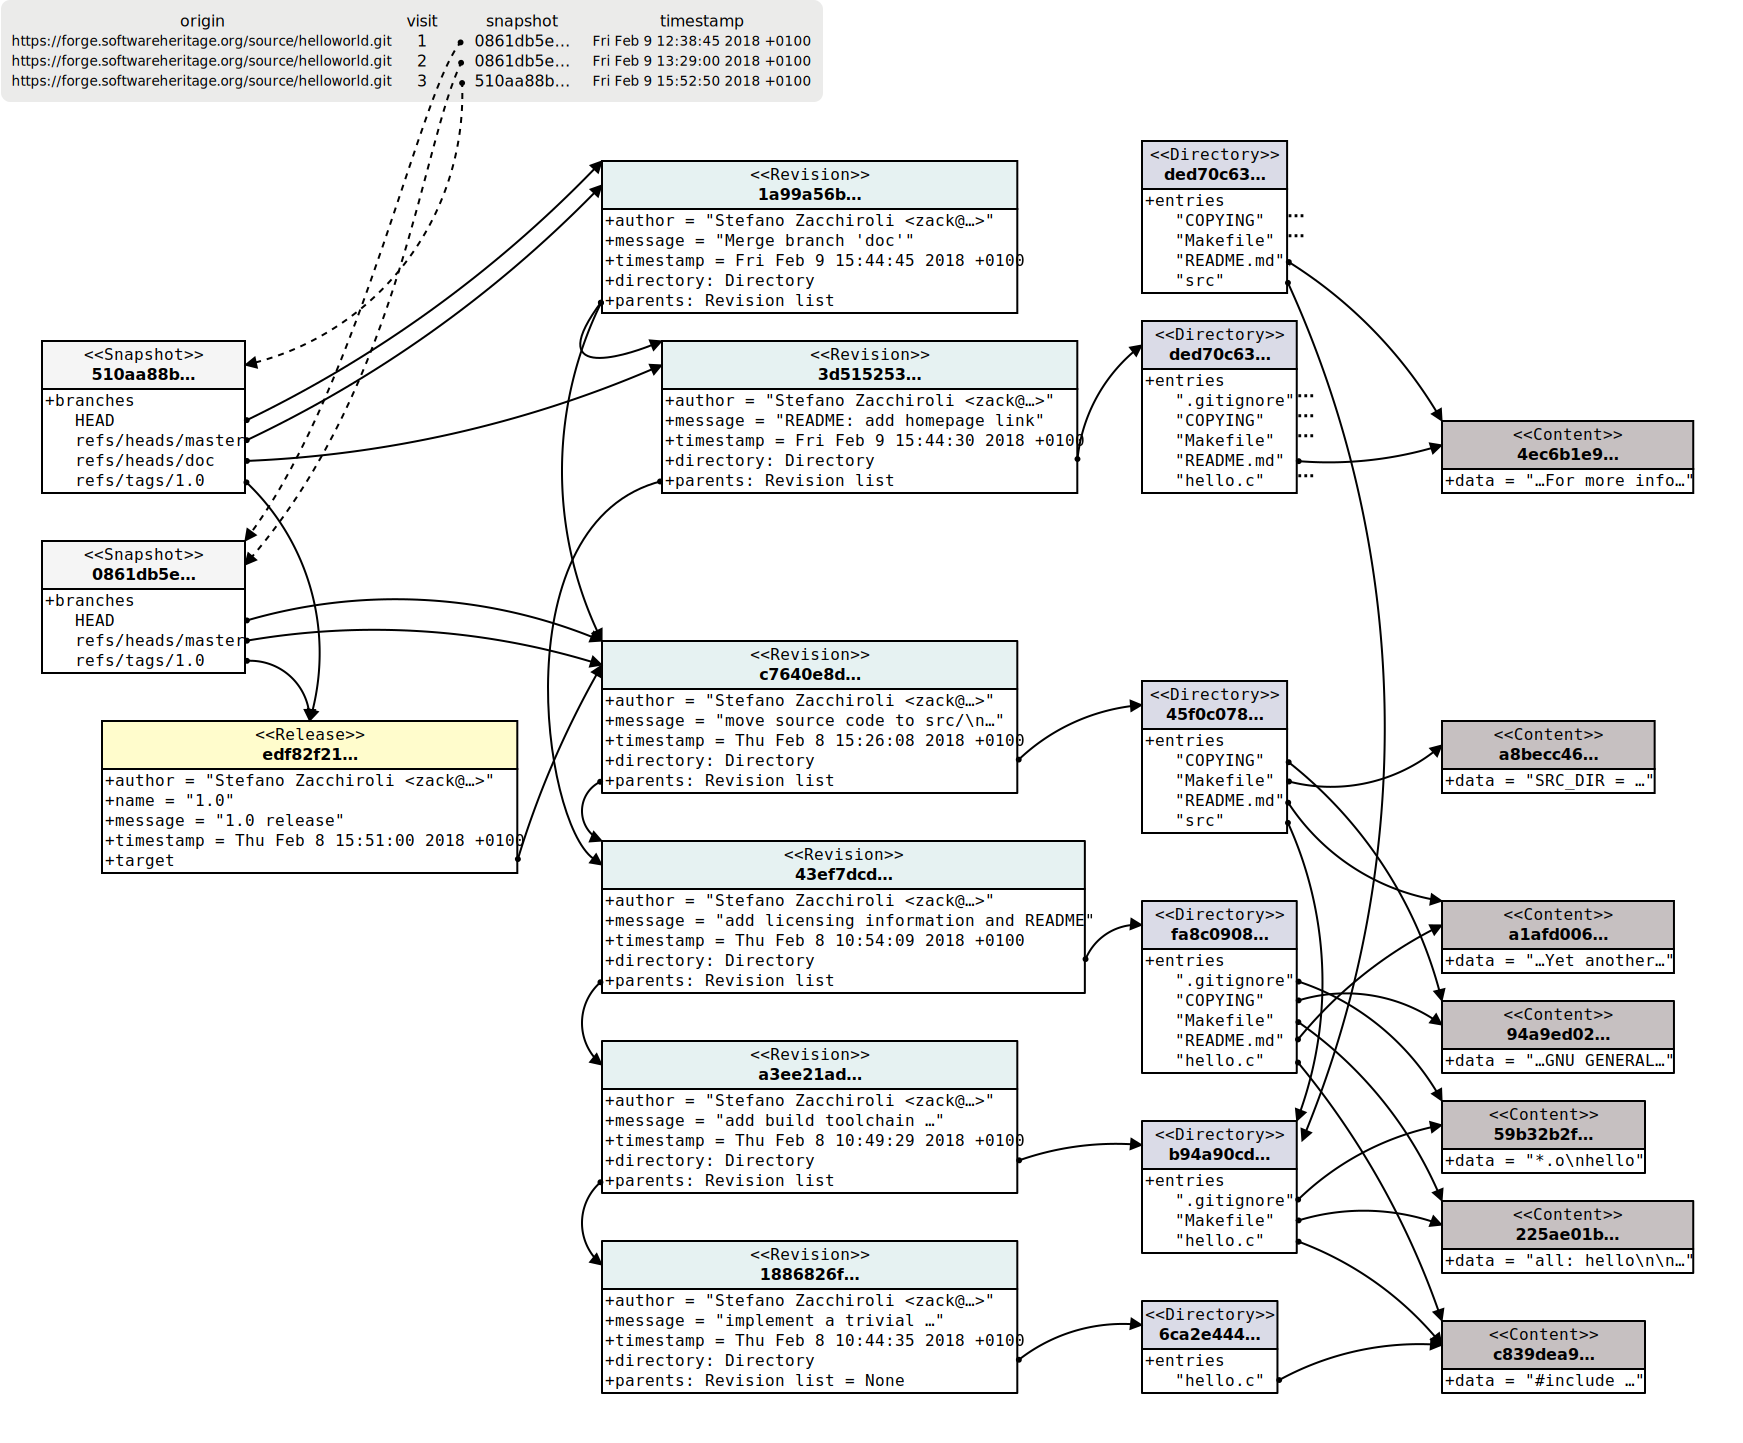
\includegraphics[height=7.5cm]{../img/swh-merkle-dag}
        \end{figure}
    \end{frame}

    % \begin{frame}
    %     \frametitle{Graph statistics}
    %     \begin{columns}
    %         \column{.50\textwidth}
    %         \begin{block}{Graph topology}
    %             \begin{itemize}
    %                 \item $\approx$ 20 billion nodes
    %                 \item $\approx$ 220 billion edges
    %             \end{itemize}
    %         \end{block}

    %         \column{.50\textwidth}
    %         \begin{block}{Software artifacts}
    %             \begin{itemize}
    %                 \item $\approx$ 150 million software projects
    %                 \item $\approx$ 2 billion commits
    %                 \item $\approx$ 10 billion source code files
    %             \end{itemize}
    %         \end{block}
    %     \end{columns}
    % \end{frame}

    % vcs
    % archive

    \section{Making Software Data Available for Mining}

    \begin{frame}
        \frametitle{Research requirements}

        \begin{block}{Identifying researchers need}
            Literature review of \textbf{54 papers} from the Mining Software
            Repositories conference (MSR 2019).
        \end{block}

        \begin{block}{Categories of requested data}
            \begin{itemize}
                \item Blobs
                \item Filesystem hierarchy (\emph{file names, directories})
                \item History graph (\emph{revisions})
                \item Content search (\emph{full-text search index})
                \item Provenance (\emph{backwards index})
                \item Commit diffs
                \item Community graph (\emph{revision authors})
                \item Dependency data
            \end{itemize}
        \end{block}
    \end{frame}

    \begin{frame}
        \frametitle{Data volume challenges}

        \begin{block}{Local analysis}
            Handling data at that scale is a hard problem for researchers:
            \begin{itemize}
                \item Data does not fit on a single machine
                \item Unusual size distribution of contents (a lot of very small files: median \textasciitilde{}3 kB) \\
                    → hard to use classical distributed storage solutions
                \item Downloading this volume of data can take months
            \end{itemize}
        \end{block}

        \begin{block}{Potential solutions}
            \begin{itemize}
                \item Sampling: access restricted amounts of data
                \item Scale-out: platform for distributed computing
                \item Scale-up: graph compression
            \end{itemize}
        \end{block}
    \end{frame}

    \begin{frame}
        \frametitle{The Vault}

        \begin{block}{}
            The \textbf{Vault}: Download single directories or entire
            repositories.
        \end{block}

        \begin{center}
            \includegraphics[width=\linewidth]{img/vault.png}
        \end{center}

        \begin{block}{}
            \begin{itemize}
                \item Retrieves the transitive closure of a
                    given object and bundles it in a tarball.
                \item Serves as a cache for downloadable tarballs.
                \item Scales up to tens of thousands of repositories
            \end{itemize}
        \end{block}
    \end{frame}

    \begin{frame}[fragile]
        \frametitle{SwhFS}

        \begin{block}{}
            The \textbf{Software Heritage Filesystem}: a virtual FUSE
            filesystem to mount the archive as a local directory.

            \begin{itemize}
                \item Useful for prototyping
                \item Easy to exploit with common CLI tools \\
                    → Local file hierarchy maps well with archived repositories
                \item Suited for small-scale experiments
            \end{itemize}

            \footnotesize
            \begin{thebibliography}{swhfs}
                \bibitem{swhfs2020} Thibault Allançon, Antoine Pietri, Stefano Zacchiroli\newblock
                The Software Heritage Filesystem (SwhFS): Integrating Source Code Archival with Development\newblock
                ICSE 2021, IEEE\newblock
            \end{thebibliography}
        \end{block}

        \begin{block}{}
            \begin{minted}{console}
$ cd archive/swh:1:dir:1fee702c7e6d14395bbf5ac3598e73bcbf97b030
$ grep -i antenna THE_LUNAR_LANDING.s | cut -f 5
# IS THE LR ANTENNA IN POSITION 1 YET
# BRANCH IF ANTENNA ALREADY IN POSITION 1
            \end{minted}
        \end{block}
    \end{frame}

    \begin{frame}
        \frametitle{The Software Heritage Graph Dataset}

        \begin{block}{}
            The \textbf{Software Heritage Graph Dataset}: a snapshot of the
            entire graph of software development (without the file contents).

            \footnotesize
            \begin{thebibliography}{msr2019}
                \bibitem{swhgraph2019} Antoine Pietri, Diomidis Spinellis, Stefano Zacchiroli\newblock
                The Software Heritage graph dataset: public software development under one roof\newblock
                Mining Software Repositories 2019\newblock
            \end{thebibliography}
        \end{block}

        \begin{block}{Formats}
            \begin{itemize}
                \item A set of \emph{relational tables} in columnar format for
                    scale-out processing
                \item A \emph{graph edges} format for use in graph databases
                    and graph analysis platforms
            \end{itemize}
        \end{block}

        \begin{block}{Availability}
            \begin{itemize}
                \item Downloadable for local use
                \item Cloud processing platforms: Amazon Athena, Azure
                    Databricks
            \end{itemize}
        \end{block}
    \end{frame}

    \begin{frame}[fragile]{Example queries}
        \begin{block}{Most frequent first commit words}
            \begin{minted}[fontsize=\small]{sql}
SELECT COUNT(*) AS c, word FROM (
  SELECT LOWER(REGEXP_EXTRACT(FROM_UTF8(
  message), 'ˆ\w+')) AS word FROM revision)
WHERE word != ''
GROUP BY word ORDER BY COUNT(*) DESC LIMIT 5;
            \end{minted}

            \begin{center}
                \begin{tabular}{rl}
                    Count & Word\\
                    \hline
                    \num{71338310} & update\\
                    \num{64980346} & merge\\
                    \num{56854372} & add\\
                    \num{44971954} & added\\
                    \num{33222056} & fix\\
                \end{tabular}
            \end{center}
        \end{block}
    \end{frame}

    \begin{frame}[fragile]{Example queries}
        \begin{columns}
            \column{0.5\textwidth}
            \begin{block}{Weekend work}
                \inputminted[fontsize=\tiny, firstline=3]{sql}{../codesamples/graph-dataset/weekend-work.sql}
            \end{block}
            \column{0.5\textwidth}
            \begin{center}
                \includegraphics[width=\linewidth]{../img/graph-dataset/weekend-work}
            \end{center}
        \end{columns}
    \end{frame}

    \begin{frame}[fragile]{Example queries}
        \begin{block}{Spark: Connected components size distribution}
            \inputminted[fontsize=\small]{sql}{../codesamples/graph-dataset/spark-cc.py}
        \end{block}

        \begin{block}{}
            \textbf{Warning}: distributed graph algorithms on Spark are very
            expensive (\textasciitilde{}5000 USD for the entire graph with
            Azure Databricks).
        \end{block}
    \end{frame}

    \section{Graph Compression and Exploitation}

    \begin{frame}
        \frametitle{Compression approach}

        \begin{block}{}
            \textbf{Objective}: Storing the \emph{entire graph of public
            software development} on a single machine.

            \footnotesize
            \begin{thebibliography}{swhgraphcomp}
                \bibitem{Boldi2020} Paolo Boldi, Antoine Pietri, Sebastiano Vigna, Stefano Zacchiroli
                \newblock Ultra-Large-Scale Repository Analysis via Graph Compression
                \newblock SANER 2020, 27th Intl. Conf. on Software Analysis, Evolution and Reengineering. IEEE
            \end{thebibliography}
        \end{block}

        \begin{block}{Advantages}
            \begin{itemize}
                \item Simpler for prototyping, no need to write distributed
                    algorithms
                \item Cheaper than scale-out processing
                \item No need to resort to sampling
                \item Allows us to run topological analyses quickly
            \end{itemize}
        \end{block}
    \end{frame}

    \begin{frame}{Background: (Web) graph compression}
        \begin{definition}[The graph of the Web]
            Directed graph that has Web pages as nodes and hyperlinks between them as
            edges.
        \end{definition}
        \begin{block}{Properties (1)}
            \begin{itemize}
                \item \alert{\alert{Locality:}} pages links to pages whose URL is lexicographically
                    similar. URLs share long common prefixes.
            \end{itemize}

            → use \alert{D-gap compression}
        \end{block}
        \begin{columns}
            \begin{column}{0.5\columnwidth}
                \begin{block}{Adjacency lists}
                    \scriptsize
                    \begin{center}
                        \begin{tabular}{rrl}
                            \alert{Node} & \alert{Outd.} & \alert{Successors}\\
                            \hline
                            \ldots{} & \ldots{} & \ldots{}\\
                            15 & 11 & 13,15,16,17,18,19,23,24,203,315,1034\\
                            16 & 10 & 15,16,17,22,23,24,315,316,317,3041\\
                            17 & 0 & \\
                            18 & 5 & 13,15,16,17,50\\
                            \ldots{} & \ldots{} & \ldots{}\\
                        \end{tabular}
                    \end{center}
                \end{block}
            \end{column}
            \begin{column}{0.50\columnwidth}
                \begin{block}{D-gapped adjacency lists}
                    \scriptsize
                    \begin{center}
                        \begin{tabular}{rrl}
                            \alert{Node} & \alert{Outdegree} & \alert{Successors}\\
                            \hline
                            \ldots{} & \ldots{} & \ldots{}\\
                            15 & 11 & 3,1,0,0,0,0,3,0,178,111,718\\
                            16 & 10 & 1,0,0,4,0,0,290,0,0,2723\\
                            17 & 0 & \\
                            18 & 5 & 9,1,0,0,32\\
                            \ldots{} & \ldots{} & \ldots{}\\
                        \end{tabular}
                    \end{center}
                \end{block}
            \end{column}
        \end{columns}
    \end{frame}

    \begin{frame}{Background: (Web) graph compression (cont.)}
        \begin{definition}[The graph of the Web]
            Directed graph that has Web pages as nodes and hyperlinks between them as
            edges.
        \end{definition}
        \begin{block}{Properties (2)}
            \begin{itemize}
                \item \alert{\alert{Similarity:}} pages that are close together in lexicographic order tend
                    to have many common successors.
            \end{itemize}
            → use \alert{reference compression}
        \end{block}
        \begin{columns}
            \begin{column}{0.47\columnwidth}
                \begin{block}{Adjacency lists}
                    \scriptsize
                    \begin{center}
                        \begin{tabular}{rrl}
                            \alert{Node} & \alert{Outd.} & \alert{Successors}\\
                            \hline
                            \ldots{} & \ldots{} & \ldots{}\\
                            15 & 11 & 13,15,16,17,18,19,23,24,203,315,1034\\
                            16 & 10 & 15,16,17,22,23,24,315,316,317,3041\\
                            17 & 0 & \\
                            18 & 5 & 13,15,16,17,50\\
                            \ldots{} & \ldots{} & \ldots{}\\
                        \end{tabular}
                    \end{center}
                \end{block}
            \end{column}
            \begin{column}{0.60\columnwidth}
                \begin{block}{Copy lists}
                    \scriptsize
                    \begin{center}
                        \begin{tabular}{rrll}
                            \alert{Node} & \alert{Ref.} & \alert{Copy list} & \alert{Extra nodes}\\
                            \hline
                            \ldots{} & \ldots{} & \ldots{} & \ldots{}\\
                            15 & 0 &  & 13,15,16,17,18,19,23,24,203,315,1034\\
                            16 & 1 & 01110011010 & 22,316,317,3041\\
                            17 &  &  & \\
                            18 & 3 & 11110000000 & 50\\
                            \ldots{} & \ldots{} & \ldots{} & \\
                        \end{tabular}
                    \end{center}
                \end{block}
            \end{column}
        \end{columns}
    \end{frame}


    \begin{frame}{Compression pipeline}
        \begin{block}{Application to the software development graph: (re)establishing locality}
            \begin{itemize}
                \item key for good compression is a node ordering that ensures locality and
                    similarity
                \item which is very much \emph{not} the case with Merkle IDs\ldots{}
                \item \ldots{}but is the case \emph{again} after BFS
            \end{itemize}
        \end{block}
        \begin{center}
            \includegraphics[width=1\linewidth]{../img/compression/compression_steps-nofiles}
        \end{center}
        \vspace{-1cm}
        \begin{itemize}
            \item \alert{MPH:} minimal perfect hash, mapping Merkle IDs to 0..N-1 integers
            \item \alert{BV compress:} Boldi-Vigna compression (based on MPH order)
            \item \alert{BFS:} breadth-first visit to renumber
            \item \alert{Permute:} update BV compression according to BFS order
        \end{itemize}
    \end{frame}

    \begin{frame}{Compression time}
        We ran the compression pipeline on the input corpus using the WebGraph
        framework
        \begin{thebibliography}{}
            \footnotesize
            \bibitem{BoVWFI} Paolo Boldi and Sebastiano Vigna.
            \newblock The WebGraph framework I: Compression techniques
            \newblock WWW 2004: 13th Intl. World Wide Web Conference. ACM
        \end{thebibliography}

        \begin{center}
            \begin{tabular}{lr}
                \alert{Step} & \alert{Wall time} (hours)\\
                \hline
                MPH & 2\\
                BV Compress & 84\\
                BFS & 19\\
                Permute & 18\\
                Transpose & 15\\
                \hline
                Total & 138 (6 days)\\
            \end{tabular}
        \end{center}

        \begin{itemize}
            \item server equipped with 24 CPUs and 750 GB of RAM
            \item RAM mostly used as I/O cache for the BFS step
            \item \emph{minimum} memory requirements are close to the RAM needed to load the
                final compressed graph in memory
        \end{itemize}
    \end{frame}

    \begin{frame}{Compression efficiency}
        \begin{block}{}
            \begin{itemize}
                \item Starting point: 6 TiB edges file
                \item Output: compressed graph containing the topology only (no
                    names or attributes)
            \end{itemize}
        \end{block}
        \begin{columns}
            \begin{column}{0.4\columnwidth}
                \begin{block}{Forward graph}
                    \begin{center}
                        \begin{tabular}{lr}
                            total size & 91 GiB\\
                            bits per edge & 4.91\\
                        \end{tabular}
                    \end{center}
                \end{block}
            \end{column}
            \begin{column}{0.4\columnwidth}
                \begin{block}{Backward graph}
                    \begin{center}
                        \begin{tabular}{lr}
                            total size & 83 GiB\\
                            bits per edge & 4.49\\
                        \end{tabular}
                    \end{center}
                    \vfill
                \end{block}
            \end{column}
        \end{columns}
        \begin{block}{Operational cost}
            The structure of a full bidirectional archive graph fits in less than 200
            GiB of RAM, for a hardware cost of \textasciitilde{}300 USD.
        \end{block}
    \end{frame}

    \begin{frame}{A domain-agnostic benchmark --- full corpus traversal}
        \begin{block}{Benchmark --- Full BFS visit}
            \begin{columns}\begin{column}{0.45\textwidth}
                \begin{center}
                    \begin{tabular}{ll}
                        \alert{Forward  graph} & \\
                        \hline
                        wall time & 1h48m\\
                        throughput & 1.81 M nodes/s\\
                                   & (553 ns/node)\\
                    \end{tabular}
                \end{center}
                \end{column}\begin{column}{0.45\textwidth}
                \begin{center}
                    \begin{tabular}{ll}
                        \alert{Backward graph} & \\
                        \hline
                        wall time & 3h17m\\
                        throughput & 988 M nodes/s\\
                                   & (1.01 µs/node)\\
                    \end{tabular}
                \end{center}
            \end{column}\end{columns}
        \end{block}
        For comparison, BFS of this graph on Spark/GraphFrames: 4 hours, 80
        nodes(!), 5000~USD.
    \end{frame}

    \begin{frame}{A domain-agnostic benchmark --- edge lookup}
        \begin{block}{Benchmark --- Edge lookup}
            random sample: 1 B nodes (8.3\% of entire graph)
            \begin{columns}\begin{column}{0.45\textwidth}
                \begin{center}
                    \begin{tabular}{ll}
                        \alert{Forward  graph} & \\
                        \hline
                        visited edges & 13.6 B\\
                        throughput & 12.0 M edges/s\\
                                   & (83 ns/edge)\\
                    \end{tabular}
                \end{center}
                \end{column}\begin{column}{0.45\textwidth}
                \begin{center}
                    \begin{tabular}{ll}
                        \alert{Backward graph} & \\
                        \hline
                        visited edges & 13.6 B\\
                        throughput & 9.45 M edges/s\\
                                   & (106 ns/edge)\\
                    \end{tabular}
                \end{center}
            \end{column}\end{columns}
        \end{block}
        Note how edge lookup time is close to DRAM random access time (50-60 ns).
    \end{frame}

    % \begin{frame}{Limitations}
    %     \begin{block}{Incrementality}
    %         \begin{itemize}
    %             \item compression is inherently \alert{not incremental}
    %             \item not an issue for most research use cases, because we analyze immutable
    %                 data dumps
    %             \item common workaround (e.g., for the Web and social networks) is to keep an
    %                 uncompressed \alert{in-memory overlay} for graph updates, and periodically
    %                 recompress
    %         \end{itemize}
    %     \end{block}
    % \end{frame}

    \begin{frame}{LLP compression}
        \begin{block}{Layered Label Propagation}
            \begin{thebibliography}{Foo Bar, 1969}
                \small \vspace{-2mm}
                \bibitem{Boldi2010} Paolo Boldi, Marco Rosa, Massimo Santini, Sebastiano Vigna
                \newblock Layered Label Propagation: A MultiResolution Coordinate-Free Ordering for Compressing Social Networks
            \end{thebibliography}
        \end{block}
        \begin{block}{}
            \begin{itemize}
                \item New algorithm to find locality information
                \item Propagates labels on random nodes to discover neighborhoods
                \item Compression requires more runtime memory (33 bytes per node)
                \item Even more impressive compression ratio (117 GiB → 77 GiB)
            \end{itemize}
        \end{block}
    \end{frame}

    \begin{frame}{Graph Attributes}
        \begin{block}{Node attributes}
            \begin{itemize}
                \item the compressed in-memory graph structure has \alert{no attributes}
                \item usual data design is to exploit the 0..N-1 integer ranges to \alert{memory map
                    \emph{node} attributes} to secondary storage (node ID →
                    node attribute)
                    \begin{itemize}
                        \item We do this for node types (mapping: 4 GiB),
                            timestamps (mapping: 149 GiB), etc.
                        \item Data structures: integer/byte arrays, front-coded
                            string lists, etc.
                    \end{itemize}
            \end{itemize}
        \end{block}
        \begin{block}{Edge attributes}
            \begin{itemize}
                \item Built-in WebGraph support for attributes on the \alert{edges} (generally integers)
                \item For file \emph{names}, we use another minimal perfect hash to map file names to integers
            \end{itemize}
        \end{block}
        \begin{block}{Disk/memory consideration}
            \begin{itemize}
                \item Labels and mappings can be either in RAM or
                    \texttt{mmap()}-ed from disk
                \item Time/memory tradeoff, depends on access patterns, intensive
                    workloads etc.
            \end{itemize}
        \end{block}
    \end{frame}

    \begin{frame}[fragile]{Graph Querying}
        \begin{block}{}
            \textbf{Option 1}: Write a traversal algorithm using low-level Java
            primitives
        \end{block}
        \begin{minted}[fontsize=\scriptsize,highlightlines={8}]{java}
HashSet<Long> visited = new HashSet<>();
Stack<Long> stack = new Stack<>();
stack.push(srcNodeId);
visited.add(srcNodeId);

while (!stack.isEmpty()) {
    long currentNodeId = stack.pop();
    LazyLongIterator it = graph.successors(currentNodeId);
    for (long neighborNodeId; (neighborNodeId = it.nextLong()) != -1; ) {
        if (!visited.contains(neighborNodeId)) {
            stack.push(neighborNodeId);
            visited.add(neighborNodeId);
        }
    }
}
        \end{minted}
        \begin{block}{}
            \begin{itemize}
                \item Very efficient but burdensome, requires local access to
                    the graph server.
                \item Most traversals are simple traversals ⇒ need for a
                    generic traversal query interface.
            \end{itemize}
        \end{block}
    \end{frame}

    \begin{frame}[fragile]
        \frametitle{Graph Querying}

        \begin{block}{}
            \textbf{Option 2}: HTTP API for simple graph traversals

            \begin{itemize}
                \item Generic remote API for graph traversals, Java/Python/aiohttp backend
                \item Limited to simple DFS from a single node (forward or
                    backward graph)
                \item Traversal types: neighbors, leaves, all nodes, all edges
                \item Supports edge type filtering
            \end{itemize}
        \end{block}

        \begin{minted}[fontsize=\scriptsize]{text}
> GET /leaves/swh:1:rev:f39d[...]2a35?direction=backward
swh:1:ori:634a2b699d442aa9abd5008f379847816f54ab85
swh:1:ori:571a86b198c6c66ef33025249f7e455b529aae65
swh:1:ori:c15194d6cb59a6d32777ca3b287ea6664d540df3
...

> GET /visit/nodes/swh:1:rev:c6df[...]fc28?edges=rel:rev,rev:rev
swh:1:rel:c6df0a7ef73ca90825f1472b8a3c5f7a2ce3fc28
swh:1:rev:c8448ff2f9234332f0bc25dc3a13031f8ab3c73c
swh:1:rev:4b63dbd4e782e74bdc050c4579381d29b4bd41c0
...
        \end{minted}
    \end{frame}

    \begin{frame}
        \frametitle{Graph Subdatasets}

        \begin{block}{Generating representative subgraphs}
            \begin{itemize}
                \item Useful for smaller-scale experimentation, prototyping
                \item Focusing analysis on a relevant subset
                \item Representative samples → transitive closure of a subset
                    of origins
                \item Use a fitted log model to estimate the size of the
                    resulting subgraph
            \end{itemize}
        \end{block}

        \begin{center}
            \includegraphics[width=.5\linewidth]{../img/graph-exploitation/subdataset_size_function_fit.pdf}
        \end{center}
    \end{frame}

    \section{Graph Topology of Software Development}

    \begin{frame}
        \frametitle{Graph Topology: Research Questions}

        \begin{block}{}
            The Software Heritage Graph Dataset materializes a \emph{network of
            relationships between software artifacts} which has not yet been
            empirically studied as a whole.
        \end{block}

        \begin{block}{Research questions}

            \begin{itemize}
                \item What is the low-level topology of the graph of software
                    development?

                    Network topology metrics: Degree distributions, connected
                    components, distance between roots and leaves, clustering
                    coefficient.

                \item What do these metrics tell us about this graph and its
                    layers?
                    \begin{itemize}
                \item Best approaches for large scale analysis?
                \item Methodological implications for software mining?
                    \end{itemize}
            \end{itemize}

            The \textbf{compressed graph framework} allows us to answer these
            questions experimentally.

            \footnotesize
            \begin{thebibliography}{swhforks}
                \bibitem{swhforks} Antoine Pietri, Guillaume Rousseau, Stefano Zacchiroli\newblock
                Determining the intrinsic structure of public software development history\newblock
                Mining Software Repositories 2020\newblock
            \end{thebibliography}
        \end{block}
    \end{frame}

    \begin{frame}
        \frametitle{Graph layers}

        \begin{block}{}
            We study the topology of the graph as a whole, but also of its
            different semantic layers:
        \end{block}

        \begin{center}
            \scalebox{0.6}{\begin{tikzpicture}[scale=0.8, label distance=1pt]
	\begin{pgfonlayer}{nodelayer}
		\node [draw, shape=ellipse, style=originfill] (origin) at (2, 2) {Origin};
		\node [draw, shape=ellipse, style=snapshotfill] (snapshot) at (2, 0) {Snapshot};
		\node [draw, shape=ellipse, style=releasefill] (release) at (2, -2) {Release};
		\node [draw, shape=ellipse, style=revisionfill] (revision) at (2, -4) {Revision};
		\node [draw, shape=ellipse, style=directoryfill] (directory) at (2, -6) {Directory};
		\node [draw, shape=ellipse, style=contentfill] (content) at (2, -8) {Blob};
		\node [style=none] (1) at (-1.25, -5.25) {};
		\node [style=none] (2) at (4, -5.25) {};
		\node [style=none] (3) at (-1.25, -8.75) {};
		\node [style=none] (4) at (4, -8.75) {};
		\node [style=none] (5) at (-1.25, 2.75) {};
		\node [style=none] (6) at (4, 2.75) {};
		\node [style=none] (7) at (-1.25, -0.75) {};
		\node [style=none] (8) at (4, -0.75) {};
		\node [style=none] (9) at (-1, -3.25) {};
		\node [style=none] (10) at (-1, -4.75) {};
		\node [style=none] (11) at (4, -4.75) {};
		\node [style=none] (12) at (4, -3.25) {};
		\node [style=none] (13) at (-1.25, -1) {};
		\node [style=none] (14) at (7, -1) {};
		\node [style=none] (15) at (-1.25, -5) {};
		\node [style=none] (16) at (7, -5) {};
		\node [style=none] (17) at (-1.5, 3) {};
		\node [style=none] (18) at (-1.5, -9) {};
		\node [style=none] (19) at (10, -9) {};
		\node [style=none] (20) at (10, 3) {};
	\end{pgfonlayer}
	\begin{pgfonlayer}{edgelayer}
		\draw [style=cluster] (5.center) to (6.center);
		\draw [style=cluster] (6.center) to (8.center);
		\draw [style=cluster] (8.center) to (7.center);
		\draw [style=cluster] (5.center) to (7.center);
		\draw [style=cluster] (13.center) to (14.center);
		\draw [style=cluster] (14.center) to (16.center);
		\draw [style=cluster] (16.center) to (15.center);
		\draw [style=cluster] (15.center) to (13.center);
		\draw [style=cluster] (9.center) to (10.center);
		\draw [style=cluster] (10.center) to (11.center);
		\draw [style=cluster] (11.center) to (12.center);
		\draw [style=cluster] (9.center) to (12.center);
		\draw [style=cluster] (1.center) to (3.center);
		\draw [style=cluster] (3.center) to (4.center);
		\draw [style=cluster] (1.center) to (2.center);
		\draw [style=cluster] (2.center) to (4.center);
		\draw [style=cluster] (17.center) to (18.center);
		\draw [style=cluster] (18.center) to (19.center);
		\draw [style=cluster] (19.center) to (20.center);
		\draw [style=cluster] (20.center) to (17.center);
		\draw [style=arrow] (origin) to (snapshot);
		\draw [style=arrow] (snapshot) to (release);
		\draw [style=arrow] (release) to (revision);
		\draw [style=arrow] (revision) to (directory);
		\draw [style=arrow] (directory) to (content);
		\draw [style=dashed arrow, draw=lightgray, bend right=60, looseness=0.75] (snapshot) to (content);
		\draw [style=dashed arrow, draw=lightgray, bend right=60, looseness=0.75] (snapshot) to (directory);
		\draw [style=dashed arrow, draw=lightgray, bend right=45] (release) to (directory);
		\draw [style=dashed arrow, draw=lightgray, bend right=45] (release) to (content);
		\draw [style=arrow, loop left, loop] (revision) to ();
		\draw [style=arrow, bend right] (directory) to (revision);
		\draw [style=arrow, loop left, loop] (directory) to ();
		\draw [style=arrow, bend right=60] (snapshot) to (revision);

        \draw [decorate, decoration={brace,raise=5pt,amplitude=10pt}] (6) to node [align=left, right=20pt, style=none] {Hosting\\ layer} (8);
        \draw [decorate, decoration={brace,raise=5pt,amplitude=5pt}] (12) to node [align=left, right=20pt, style=none] {Commit\\ layer} (11);
        \draw [decorate, decoration={brace,raise=5pt,amplitude=10pt}] (2) to node [align=left, right=20pt, style=none] {Filesystem\\ layer} (4);
        \draw [decorate, decoration={brace,raise=5pt,amplitude=10pt}] (14) to node [align=left, right=20pt, style=none] {History\\ layer} (16);
        \draw [decorate, decoration={brace,raise=5pt,amplitude=10pt}] (20) to node [align=left, right=20pt, style=none] {Full graph} (19);
	\end{pgfonlayer}
\end{tikzpicture}
}
        \end{center}
    \end{frame}

    \begin{frame}
        \frametitle{Average degree}

        \begin{table}
            \centering
            \begin{tabular}[t]{l S[table-format=3.3]}
                \textbf{Dataset} & \textbf{Average degree} \\
                \hline
                \textbf{swh-2020-history}    & 1.021 \\
                \textbf{swh-2020-commit}     & 1.022 \\
                \textbf{swh-2020-hosting}    & 3.39 \\
                bitcoin-2013 & 6.4 \\
                dblp-2011 (Co-authorship)       & 6.8 \\
                \textbf{swh-2020}            & 11.0 \\
                \textbf{swh-2020-filesystem} & 12.1 \\
                twitter-2010      & 35.2 \\
                clueweb12                    & 43.1 \\
                uk-2014 (Web)               & 60.4 \\
                fb-2011 (Facebook)          & 169.0 \\
            \end{tabular}
        \end{table}
    \end{frame}

    \begin{frame}
        \frametitle{Degree distributions: full graph}
        \begin{figure}
            \begin{subfigure}{.49\textwidth}
                \centering
                \includegraphics[width=\linewidth]{../img/topology/inout/full_in}
                \caption{In-degrees.}
            \end{subfigure}\hfill
            \begin{subfigure}{.49\textwidth}
                \centering
                \includegraphics[width=\linewidth]{../img/topology/inout/full_out}
                \caption{Out-degrees.}
            \end{subfigure}
        \end{figure}
    \end{frame}

    \begin{frame}
        \frametitle{Degree distributions: filesystem layer}
        \begin{figure}
            \begin{subfigure}{.49\textwidth}
                \centering
                \includegraphics[width=\linewidth]{../img/topology/inout/dir+cnt_in}
                \caption{In-degrees.}
            \end{subfigure}\hfill
            \begin{subfigure}{.49\textwidth}
                \centering
                \includegraphics[width=\linewidth]{../img/topology/inout/dir+cnt_out}
                \caption{Out-degrees.}
            \end{subfigure}
        \end{figure}

        \begin{block}{}
            Scale invariance, no characteristic degree (diverging average).
        \end{block}
    \end{frame}

    \begin{frame}
        \frametitle{Degree distributions: commit layer}
        \begin{figure}
            \begin{subfigure}{.49\textwidth}
                \centering
                \includegraphics[width=\linewidth]{../img/topology/inout/rev_in}
                \caption{In-degrees (``fork-degrees'').}
            \end{subfigure}\hfill
            \begin{subfigure}{.49\textwidth}
                \centering
                \includegraphics[width=\linewidth]{../img/topology/inout/rev_out}
                \caption{Out-degrees (``merge-degrees'').}
            \end{subfigure}
        \end{figure}

        \begin{block}{}
            Characteristic degrees due to development patterns.
        \end{block}
    \end{frame}

    \begin{frame}
        \frametitle{Distance between roots and leaves}
        \begin{figure}
            \begin{subfigure}{.49\textwidth}
                \centering
                \includegraphics[width=\linewidth]{../img/topology/shortestpath/dir+cnt}
                \caption{Filesystem layer}
            \end{subfigure}\hfill
            \begin{subfigure}{.49\textwidth}
                \centering
                \includegraphics[width=\linewidth]{../img/topology/shortestpath/rev}
                \caption{Commit layer}
            \end{subfigure}
        \end{figure}
    \end{frame}

    \begin{frame}
        \frametitle{Connected components}
        \begin{figure}
            \begin{subfigure}{.49\textwidth}
                \centering
                \includegraphics[width=0.9\linewidth]{../img/topology/connectedcomponents/dir+cnt}
                \caption{Filesystem layer}
            \end{subfigure}\hfill
            \begin{subfigure}{.49\textwidth}
                \centering
                \includegraphics[width=0.9\linewidth]{../img/topology/connectedcomponents/rev}
                \caption{Commit layer}
            \end{subfigure}
        \end{figure}

        \begin{center}
            \begin{tabular}[t]{l r r r}
                \textbf{Layer} & \textbf{\# of WCC}
                               & \textbf{Size of largest WCC}
                               & \textbf{\% of nodes in largest}
                               \\
                               \hline
                Full graph       & \num{33104255}  & \num{18902683142} & 97.79\% \\
                Filesystem layer & \num{46286502}  & \num{16565521611} & 97.16\% \\
                Commit layer     & \num{88031649}  & \num{51543944}    & 2.61\% \\
            \end{tabular}
        \end{center}
    \end{frame}

    \begin{frame}
        \frametitle{Takeways: filesystem / commit layer duality}

        \begin{block}{}
            The filesystem and commit layers have almost opposite topological
            properties.
        \end{block}

        \begin{columns}
            \column{0.5\columnwidth}
            \begin{block}{Filesystem layer}
                \begin{itemize}
                    \item Dense, non-partitionable (giant WCC)
                    \item Characteristic depth
                    \item Arbitrary outdegree
                \end{itemize}
                \begin{center}
                    \scalebox{0.7}{\begin{tikzpicture}
	\begin{pgfonlayer}{nodelayer}
		\node [style=none] (9) at (-3.5, 1.5) {};
		\node [style=none] (10) at (1.5, 1.5) {};
		\node [style=none] (11) at (1.5, 2) {};
		\node [style=none] (12) at (1.5, 5) {};
		\node [style=directory] (13) at (0, 5) {};
		\node [style=directory] (14) at (-1, 4) {};
		\node [style=directory] (15) at (0.5, 4) {};
		\node [style=content] (16) at (-2.25, 3) {};
		\node [style=content] (17) at (-1.5, 3) {};
		\node [style=content] (18) at (-0.75, 3) {};
		\node [style=directory] (19) at (0.5, 3) {};
		\node [style=content] (20) at (0, 2) {};
		\node [style=content] (22) at (-3, 3) {};
		\node [style=content] (23) at (1, 2) {};
	\end{pgfonlayer}
	\begin{pgfonlayer}{edgelayer}
		\draw [style=dashed arrow] (12.center) to (11.center);
		\draw [style=arrow] (13) to (14);
		\draw [style=arrow] (13) to (15);
		\draw [style=arrow] (15) to (19);
		\draw [style=arrow] (14) to (18);
		\draw [style=arrow] (14) to (17);
		\draw [style=arrow] (19) to (20);
		\draw [style=arrow] (19) to (23);
		\draw [style=arrow] (14) to (16);
		\draw [style=arrow] (14) to (22);
		\draw [style=dashed arrow] (12.center) to node [right, align=left] {Characteristic\\depth} (11.center);
		\draw [decorate, decoration={brace,amplitude=10pt}] (10.center) to node [align=center, below=10pt] {Arbitrary\\outdegree} (9.center);
	\end{pgfonlayer}
\end{tikzpicture}
}
                \end{center}
            \end{block}

            \column{0.5\columnwidth}
            \begin{block}{Commit layer}
                \begin{itemize}
                    \item Sparse, partitionable (max WCC = 3\%)
                    \item Arbitrary depth
                    \item Characteristic outdegree (degenerate)
                \end{itemize}
                \begin{center}
                    \scalebox{0.5}{\begin{tikzpicture}
	\begin{pgfonlayer}{nodelayer}
		\node [style=revision] (0) at (0, 0) {};
		\node [style=revision] (1) at (0, 1) {};
		\node [style=revision] (2) at (0, 2) {};
		\node [style=revision] (3) at (0, 3) {};
		\node [style=revision] (4) at (1, 2.5) {};
		\node [style=revision] (5) at (1, 1.5) {};
		\node [style=revision] (6) at (0, 4) {};
		\node [style=revision] (7) at (0, 5) {};
		\node [style=revision] (8) at (1, 3.5) {};
		\node [style=none] (9) at (-0.5, -0.5) {};
		\node [style=none] (10) at (1.5, -0.5) {};
		\node [style=none] (11) at (1.5, 0) {};
		\node [style=none] (12) at (1.5, 5) {};
	\end{pgfonlayer}
	\begin{pgfonlayer}{edgelayer}
		\draw [style=arrow] (1) to (0);
		\draw [style=arrow] (5) to (1);
		\draw [style=arrow] (2) to (1);
		\draw [style=arrow] (4) to (5);
		\draw [style=arrow] (3) to (2);
		\draw [style=arrow] (6) to (3);
		\draw [style=arrow] (3) to (4);
		\draw [style=arrow] (7) to (6);
		\draw [style=arrow] (8) to (4);
		\draw [style=dashed arrow] (12.center) to (11.center);
		\draw [style=dashed arrow] (12.center) to node [right, align=left] {Arbitrary\\depth} (11.center);
        \draw [decorate, decoration={brace,amplitude=10pt}] (10.east) to node [align=center, below=10pt] {Characteristic\\outdegree} (9.west);
	\end{pgfonlayer}
\end{tikzpicture}
}
                \end{center}
            \end{block}
        \end{columns}
    \end{frame}

    \begin{frame}
        \frametitle{Takeaways: implications for software mining research}

        \begin{block}{Layers}
            \begin{itemize}
                \item Large disparity in the low-level structure of layers
                \item Important to study layers separately to understand
                    the graph structure
            \end{itemize}
        \end{block}

        \begin{block}{Methodology}
            \begin{itemize}
                \item High kurtosis / propensity to produce outliers
                \item No obvious rule to ``filter'' outliers in many
                    distributions
                \item Highlights the importance of exhaustive approaches
            \end{itemize}
        \end{block}

        \begin{block}{Distributed analysis}
            \begin{itemize}
                \item No natural partitioning in small connected components
                \item Need for more subtle approaches (modular decomposition?)
            \end{itemize}
        \end{block}
    \end{frame}

    \section{Identification of Software Forks}

    \begin{frame}
        \frametitle{Why study software forks?}

        \begin{block}{}
            \begin{itemize}
                \item Getting a high-level view of how the graph is organized
                    in software projects
                \item Key research direction in software health and software
                    evolution
                    \begin{itemize}
                        \item Finding active and maintained projects
                        \item Understanding ``Hard'' and ``development'' forks
                        \item Identifying criteria for successful forks
                    \end{itemize}
                \item The compressed graph allows us to run exhaustive
                    quantitative studies on software forks
            \end{itemize}

            \footnotesize
            \begin{thebibliography}{swhforks}
                \bibitem{swhforks} Antoine Pietri, Guillaume Rousseau, Stefano Zacchiroli\newblock
                Forking Without Clicking: on How to Identify Software Repository Forks\newblock
                Mining Software Repositories 2020\newblock
            \end{thebibliography}
        \end{block}
    \end{frame}

    \begin{frame}
        \frametitle{Previous approaches for studying forks}

        \begin{block}{}
            \begin{itemize}
                \item Historically, studies have relied on forge-specific
                    metadata: relationships created by pressing the "fork"
                    button
                    \begin{center}
                        \includegraphics[width=2cm]{img/forkbutton}
                    \end{center}
                \item Github provides a \textbf{directed} graph of forks to parent
                    repositories
                    \begin{center}
                        \includegraphics[width=7cm]{img/forknetwork}
                    \end{center}
            \end{itemize}
        \end{block}

        \begin{block}{Biases}
            \begin{itemize}
                \item Restricted to intra-forge forks
                \item No cross-VCS information
                \item No ``manual forks''
            \end{itemize}
        \end{block}
    \end{frame}

    \begin{frame}
        \frametitle{Intrinsic forks}
        \begin{block}{Concept}
            \begin{center}
                \begin{tikzpicture}[every node/.append style={cloud,draw,very thick,align=center}]
                    \node[cloud puffs=50, aspect=7] (cloud){%
                        \textbf{Intrinsic forks} are software projects\\
                        with \textbf{shared development history}.
                    };
                \end{tikzpicture}
            \end{center}

            \begin{itemize}
                \item Identified by intrinsic DVCS information
                    \begin{itemize}
                        \item Shared commits
                        \item Shared root directories
                        \item \ldots
                    \end{itemize}
                \item Includes projects for which no forge-level metadata is present
            \end{itemize}
        \end{block}

        \begin{block}{Research question}
            How do forge forks compare to forks defined by shared development
            history?
        \end{block}
    \end{frame}

    \begin{frame}{Methodology}
        \begin{block}{Fork networks}
            \begin{center}
                Finding all the networks of intrinsic forks

                $\approx$

                Finding all the \textbf{connected components} in the
                undirected subgraph of repositories, branches, tags and commits.
            \end{center}
        \end{block}

        \begin{block}{Experimental design}
            \begin{itemize}
                \item List common repositories in Software Heritage and GitHub
                    (through GHTorrent)
                \item Extract the relevant subgraphs
                    \begin{itemize}
                        \item \textbf{Software Heritage}: hosting + history
                            layers (development graph)
                        \item \textbf{GHTorrent}: repositories → repositories (fork graph)
                    \end{itemize}
                \item Compute the connected components ⇒ \textbf{fork networks}
                \item Count the number of repositories in each fork network
            \end{itemize}
        \end{block}
    \end{frame}

    \begin{frame}
        \frametitle{Fork network results}
        \begin{center}
            \includegraphics[width=0.6\linewidth]{../img/forks/fork-network-freq-distribution.pdf}
        \end{center}
        \begin{block}{}
            \begin{itemize}
                \item \textbf{+8\% new forks discovered} (shared-commit forks)
                \item Large proportion of the repositories merged in giant
                    components
            \end{itemize}
        \end{block}
    \end{frame}

    \begin{frame}
        \frametitle{Fork cliques}
        \begin{block}{}
            \begin{itemize}
                \item By transitivity, fork networks cluster together
                    repositories which are not direct forks of each other
                \item This is in large part responsible for the giant connected
                    components
                \item Need a more restrictive definition for quantitative
                    comparisons
            \end{itemize}
        \end{block}

        \begin{block}{Fork cliques}
            Set of repositories which are \emph{all forks of each other}.
        \end{block}

        \begin{block}{Fork p-cliques}
            Partition function of the graph based on fork cliques (without
            duplicates)
        \end{block}
    \end{frame}

    \begin{frame}
        \frametitle{Fork network results}
        \begin{center}
            \includegraphics[width=0.6\linewidth]{../img/forks/fork-clique-partition-freq-distribution.pdf}
        \end{center}
        \begin{block}{}
            \begin{itemize}
                \item Positive difference ⇒ more exhaustive identification of
                    forks
                \item Distribution similarity ⇒ Matches developers'
                    expectations of what a fork is
            \end{itemize}
        \end{block}
    \end{frame}


    \section{Conclusion}

    \begin{frame}
        \frametitle{Academic contributions}

        \begin{block}{Contextualization}
            \begin{itemize}
                \item Literature review: identify research needs
                \item Roadmap to universal software mining
            \end{itemize}
        \end{block}

        \begin{block}{Making software artifacts data available}
            \begin{itemize}
                \item Small scale: Vault, SwhFS
                \item Scale-out: Graph dataset
                \item Scale-up: Graph compression \& exploitation
            \end{itemize}
        \end{block}

        \begin{block}{Empirical studies on the graph structure}
            \begin{itemize}
                \item Low-level: topological properties
                \item High-level: structure of forks
            \end{itemize}
        \end{block}
    \end{frame}

    \begin{frame}
        \frametitle{Empirical findings \& impact on software mining}
        \begin{block}{Topology}
            \begin{itemize}
                \item Disparity between graph layers
                \item Graph cannot be partitioned naturally
                \item No sound way to filter outliers
            \end{itemize}
        \end{block}
        \begin{block}{Forks}
            \begin{itemize}
                \item Forks can be identified more exhaustively with shared
                    development history
                \item They qualitatively fit established notions of what constitutes a ``fork''
            \end{itemize}
        \end{block}
    \end{frame}

    \begin{frame}
        \frametitle{Future work}

        \begin{block}{}
            \begin{itemize}
                \item Incremental graph compression
                \item Expressive remote graph querying
                \item Graph partitioning techniques for sharding (modular
                    decomposition?)
                \item Derived graphs (community graphs, diff graphs, …)
            \end{itemize}
        \end{block}
    \end{frame}

    \begin{frame}
        \frametitle{Thanks!}

        \begin{block}{}
            \emph{All} this work is open \{source, data, access, …\}.

            \url{https://forge.softwareheritage.org}
            \hfill
            \url{https://github.com/seirl/thesis}
        \end{block}

        \begin{block}{}
            \tiny
            \begin{itemize}
                \item \fullcite{swh-benevol2018-universal-analysis}
                \item \fullcite{swh-msr2019-dataset}
                \item \fullcite{msr-2020-challenge}
                \item \fullcite{saner-2020-swh-graph}
                \item \fullcite{swh-msr2020-forking}
                \item \fullcite{msr-2020-topology}
                \item \fullcite{swh-2021-swhfs}
            \end{itemize}
        \end{block}
    \end{frame}
\end{document}
